\documentclass[french,10pt,a4paper]{report}
\usepackage [utf8]{inputenc}
\usepackage [T1] {fontenc}
\usepackage{amsmath}
\usepackage{amsfonts}
\usepackage{amssymb}
\usepackage{graphicx}
\usepackage{xcolor}
\usepackage{hyperref}
\usepackage{caption}

\begin{document}
\definecolor{bb}{rgb}{0.0, 0.0, 1.0}
\definecolor{rr}{rgb}{1.0, 0.0, 0.0}
\definecolor{gg}{rgb}{0.0, 1.0, 0.0}
\definecolor{rb}{rgb}{1.0, 0.0, 1.0}
\begin{titlepage}
  \begin{center}
  	{\LARGE{ Université Paris 8 Vincennes – Saint-Denis}}\\[6cm]
    {\Large Rapport finale du cours réalisation d'application}\\[0.5cm]
    {\rule{\linewidth}{0.5mm}\\}
    { \huge \textbf{Jeu d'aventure \& \\ gestionnaire de stock}\\}
    {\rule{\linewidth}{0.5mm}\\[1cm]} 
    \end{center}
	\vfill
  	\begin{flushleft}
        \textbf{Réaliser par le groupe 1:}\\
        \textbf{
		\hspace{4cm}\textit{Anis} CHALI\\      		
      	\hspace{4cm}\textit{Habib} BALIT\\
      	\hspace{4cm}\textit{Sofiane} AIT EL DJOUDI\\
      	\hspace{4cm}\textit{Micipsa} SADJI\\
      	\hspace{4cm}\textit{Alycia} KARA\\[1cm]
        	\textbf{Encadreur :}\\
        	\hspace{4cm} M. \textit{Pierre} Lefebvre}\\[1cm]
  	\end{flushleft}
  	\begin{center}
	  	{\large 9 Mai 2019}  	
  	\end{center}
\end{titlepage}
\tableofcontents
\newpage
\chapter{Jeu d'aventure}
\section{\textcolor{rr}{Itération 1 :}}
\subsection{\textcolor{bb}{Exercice 7.1 :}}
\textbf{Que fait cette application?}\\
L’application est un jeu d’aventure basé sur du texte écrit  en lignes de commandes.\\
\textbf{Quelles commandes le jeu accepte-t-il?}\\
Le jeu accepte les commandes: help, go, quitte.\\
\textbf{Que fait chaque commande?}
\begin{itemize}
\item \textbf{Help :} Imprime des informations d'aide. Nous imprimons ici un message de bienvenu et une liste des
	mots de commande.
\item \textbf{go :} Essayez d'aller dans une direction. S'il y a une sortie, entrez la nouvelle salle, 	sinon affiche un message d'erreur.
\item \textbf{quitte :} Vérifie le reste de la commande pour voir si nous avons vraiment quitté la partie.\\
	Retour true, si cette commande quitte le jeu, false sinon.
\end{itemize}
\textbf{Combien de pièces y a-t-il dans le scénario?}\\
Il y a  5 pièces.
\begin{center}
	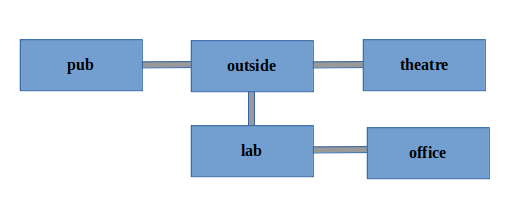
\includegraphics[scale=0.5]{captures/it1_1.png}
	\captionof{figure}{cartes des 5 pièces}
\end{center}

\subsection{\textcolor{bb}{Exercice 7.2 :}}
\textbf{Game.java :}\\
Cette classe est la classe principale de l'application "World of Zuul".\\
Pour jouer à ce jeu, créez une instance de cette classe et appeler la méthode "play" .\\
Cette classe principale crée et initialise toutes les autres, elle crée le parseur et toutes les chambres, et démarre le jeu.\\
\textbf{Room.java :}\\
Une "salle" représente un endroit dans le décor du jeu, elle est connectée à d'autres salles via des sorties. Les sorties sont étiquetées nord, est, sud, ouest. Pour chaque direction, la pièce stocke une référence de la pièce voisine, ou null s'il n'y a pas de sortie dans cette direction.\\
\textbf{Command.java :}\\
Cette classe contient des informations sur une commande émise par l'utilisateur.
Une commande est actuellement composée de deux chaînes: un mot de commande et un autre. \\
La façon dont ceci est utilisé est:
\begin{itemize}
\item Les commandes sont déjà vérifiées pour être valide.
\item Le mot de commande :  Si l'utilisateur écrit une commande non valide (un mot 	qui n'est pas connu) alors le mot de commande est  null.
\item Si la commande n'a qu'un mot, le deuxième mot est  null.
\end{itemize}
\textbf{Parser.java :}\\
Chaque fois qu'il est appelé, il lit une ligne du terminal et
tente d'interpréter la ligne comme une commande de deux mots. Il retourne la commande en tant qu'objet de la classe Command.\\
Le parseur possède un ensemble de mots de commande connus. Il vérifie les entrées de l'utilisateur avec les commandes connues, et si l'entrée n'est pas une des commandes connues, elle retourne un objet de commande qui est marqué comme une commande inconnue.\\
\textbf{CommandWords.java :}\\
Cette classe contient une énumération de tous les mots de commande connus du jeu.\\
Il est utilisé pour reconnaître les commandes au fur et à mesure de leur saisie.

\subsection{\textcolor{bb}{Exercice 7.2.1 :}}
Fait.

\subsection{\textcolor{bb}{Exercice 7.3 :}}
Pour l’instant on a imaginé un personnage qui  se balade dans une cité égyptienne ancienne, scénario  à développer prochainement…

\subsection{\textcolor{bb}{Exercice 7.3.2 :}}
\begin{center}
	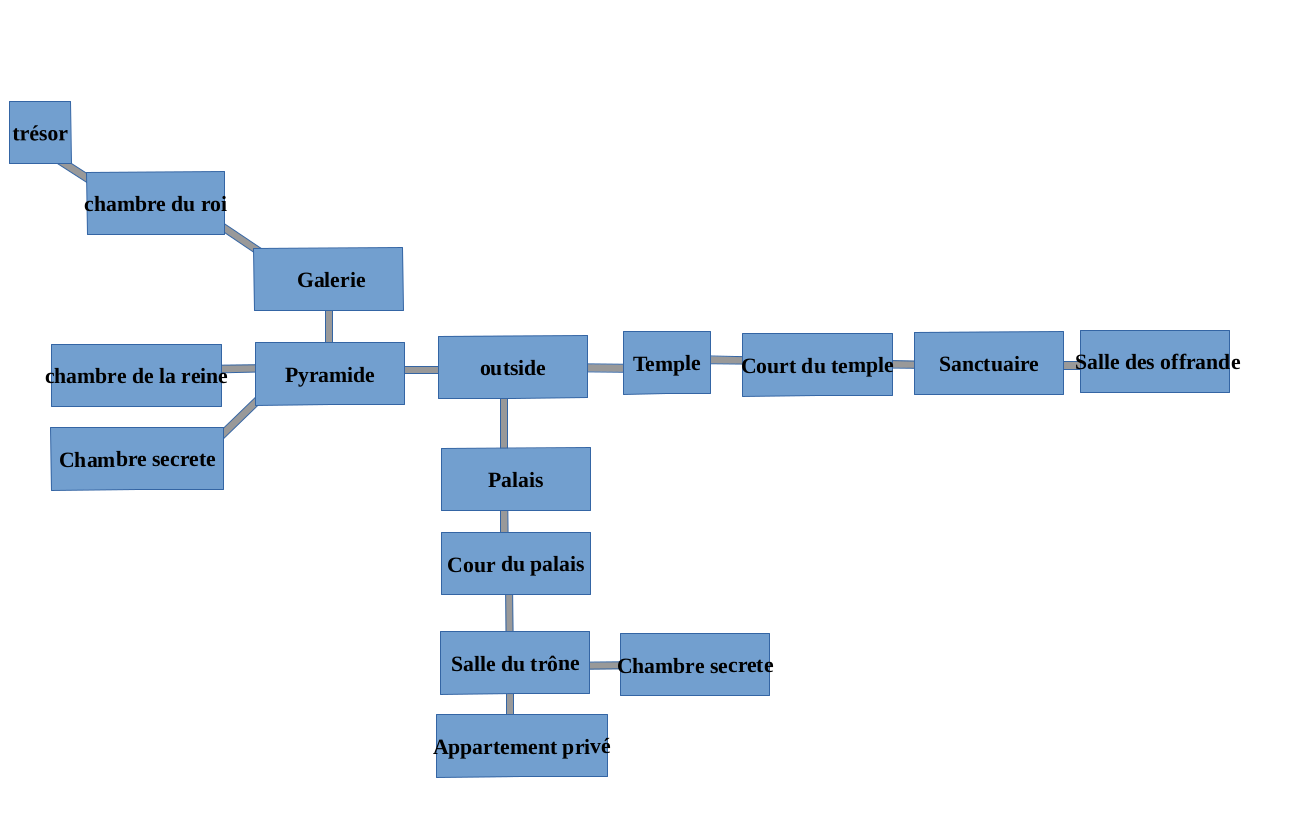
\includegraphics[scale=0.3]{captures/it1_2.png}
	\captionof{figure}{Le plan du scénario}
\end{center}

\subsection{\textcolor{bb}{Exercice 7.4 \& Exercice 7.17.2 :}}
Les modifications ont été apporté directement au code.


\section{\textcolor{rr}{Itération 2 :}}
\subsection{\textcolor{bb}{Exercice7.18 :}}
L’ajout de getCommandList dans la classe CommandWords.java ansi tous les classes correspondantes.
\begin{center}
	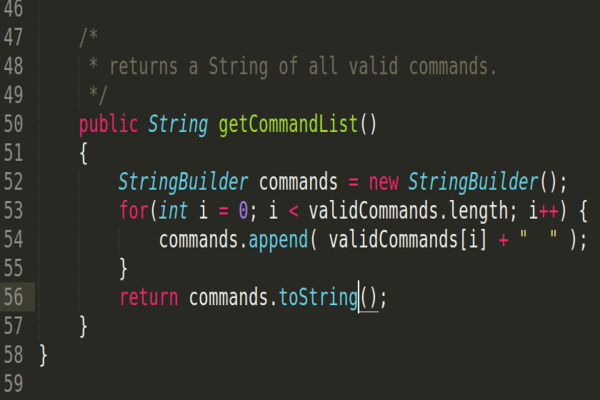
\includegraphics[scale=0.3]{captures/it2_1.png}
\end{center}

\subsection{\textcolor{bb}{Exercice 7.18.1 :}}


\subsection{\textcolor{bb}{Exercice 7.18.2 :}}
Modification de la méthode Room.getExitString() ; dans la classe Romm.java ou on modifier les variables de types String par le type StringBuilder, apres on a apporter tous les modifications nécessaire pour le reste du code.
\begin{center}
	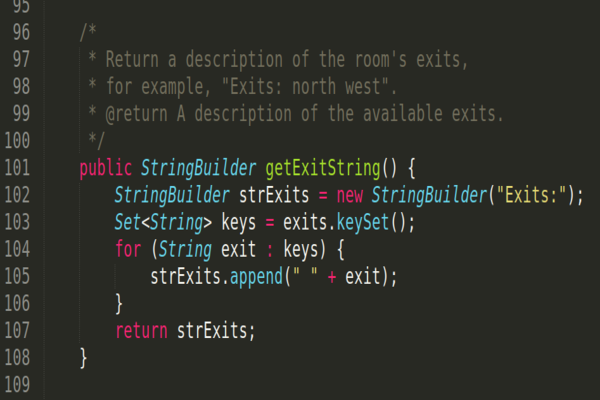
\includegraphics[scale=0.3]{captures/it2_2.png}
\end{center}
\textbf{StringBuilder :}\\Une séquence de caractères mutable. Cette classe fournit une API compatible avec StringBuffer, mais sans garantie de synchronisation. Cette classe est conçue pour une utilisation en remplacement immédiat StringBuffer dans les endroits où le tampon de chaîne était utilisé par un seul thread (comme c'est généralement le cas). Dans la mesure du possible, il est recommandé d'utiliser cette classe plutôt StringBuffer que plus rapidement, dans la plupart des cas.\\
Les principales opérations sur a StringBuilder sont les méthodes append and insert, qui sont surchargées de manière à accepter des données de tout type.

\subsection{\textcolor{bb}{Exercice 7.18.3 :}}
On a chercher une image différente pour chaque Room qui corresponds bien à notre scénario.

\subsection{\textcolor{bb}{Exercice 7.18.4 :}}
\textbf{Le titre du jeu :} \textit{\textcolor{gg}{la cité des pharaons}}.\\
Ajouter ou code, dans las classe GameEngine.java dans la methode createGUI() ;\\
myFrame = new JFrame(\textcolor{gg}{" la cité des pharaons."});

\subsection{\textcolor{bb}{Exercice 7.18.5 :}}
Pour avoir accès aux objets Room depuis n'importe quelle classe, on a créer une HashMap contenant toutes les Room (associées à leur nom) dans la classe GameEngine.java. Il suffira alors de la passer en paramètre, en cas de besoin.
\\
\textcolor{gg}{private} \textcolor{bb}{HashMap$<$ String, Room$>$} rooms;

\subsection{\textcolor{bb}{Exercice 7.18.6 :}}
Étude du projet zuul-withimages pour comprendre son fonctionnement global et intégrer dans son jeu (sans régression bien sûr ! notamment en ce qui concerne la généricité des collections : il ne doit subsister aucun warning/avertissement !) cette nouvelle conception qui permettra d'opter éventuellement par la suite pour une interface graphique plus élaborée.\\
On a opter pour se projet avant de commence cette itération 2.

\subsection{\textcolor{bb}{Exercice 7.18.7 :}}
Les interfaces EventListener permettent de définir les traitements en réponse à des événements utilisateurs généré par un composant. Une classe doit contenir une interface auditrice pour chaque type d'événements à traiter.\\
\textbf{AddActionListener():}\\
Cette méthode permet de préciser la classe qui va gérer l'événement utilisateur de type ActionListener du bouton. Cette classe doit impérativement implémenter l'interface de type EventListener correspondante soit dans notre cas ActionListener. L'instruction this indique que la classe elle même recevra et gérera l'événement utilisateur.\\
\textbf{actionPerformed() :}\\
L'apparition d'un événement utilisateur généré par un composant doté d'un auditeur appelle automatiquement une méthode qui ici  actionPerformed() . Cette dernière doit se trouver dans la classe référencée dans l'instruction qui lie l'auditeur au composant. Dans notre jeu, cette méthode doit être située dans la même classe parce que c'est l'objet lui-même qui est spécifié avec l'instruction this. 


\subsection{\textcolor{bb}{Exercice 7.18.8 :}}
On a ajouter plusieurs boutons qui correspondant ou différents commands :
\begin{center}
\begin{minipage}{0.4\textwidth}
	\begin{flushleft}
		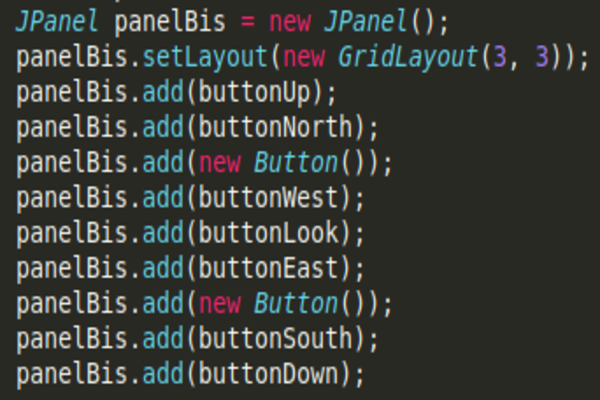
\includegraphics[scale=0.2]{captures/it2_3.png}
	\end{flushleft}
\end{minipage}
\begin{minipage}{0.4\textwidth}
	\begin{flushright}
		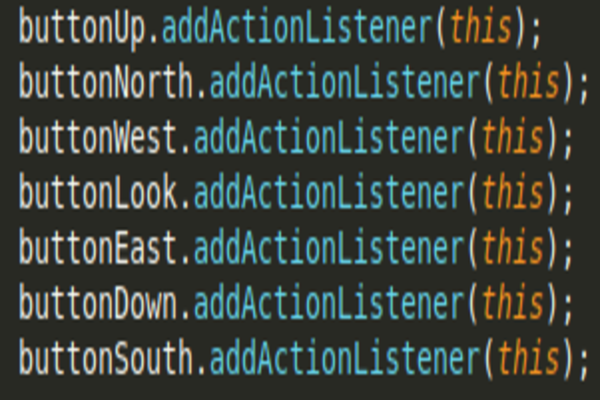
\includegraphics[scale=0.2]{captures/it2_4.png}
	\end{flushright}
\end{minipage}
\begin{minipage}{0.4\textwidth}
	\begin{center}
		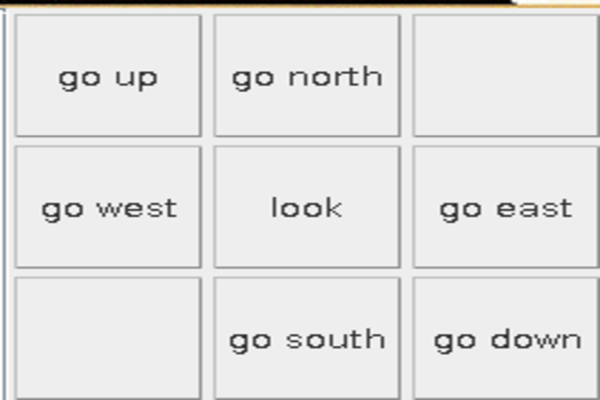
\includegraphics[scale=0.2]{captures/it2_5.png}
	\end{center}
\end{minipage}
\end{center}

\subsection{\textcolor{bb}{Exercice 7.19 \& Exercice 7.19.1 :}}
MVC fait optionnel.

\subsection{\textcolor{bb}{Exercice 7.19.2 :}}
Incorporation dans le jeu de une image différente pour chaque Room est FAIT.

\subsection{\textcolor{bb}{Exercice 7.20 :}}
On a définit pour chaque chambre un nombre d’objet aléatoire entre 3 et 5 dans chaque chambre par met un nombre définit de objets. Pour chaque objet  on associer un prix et un poids.
\begin{center}
	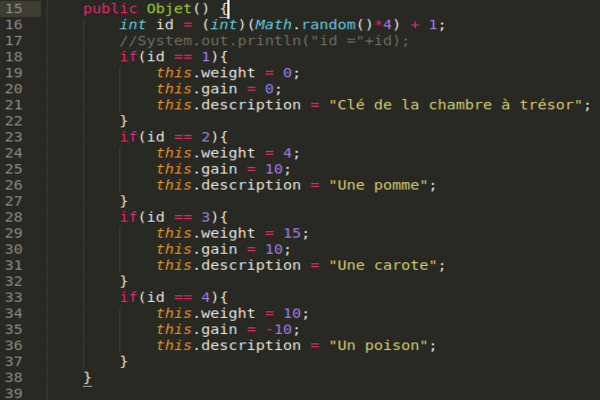
\includegraphics[scale=0.4]{captures/it2_6.png}
\end{center}

\subsection{\textcolor{bb}{Exercice 7.21 :}}
Les informations sur un objet présent dans une pièce doivent-elles être produit : on appelle seulement la méthode de l’objet getDescription() ;\\
La classe qui doit produire la chaîne décrivant l'élément : la classe Objet.java.\\
La classe qui devrait l'imprimer : la classe Room.java, car dans chaque Room j’ai un hasmap d’objet.

\subsection{\textcolor{bb}{Exercice 7.22 :}}
On utilise ici une hashMap d’objet pour chaque chambre et dans le constructeur de chaque chambre  on appelle une méthode, qui affecte un nombre d’objet aléatoire à la chambre :
\begin{center}
	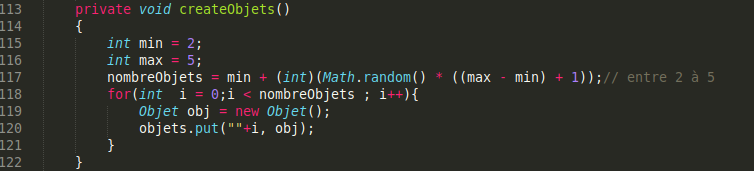
\includegraphics[scale=0.4]{captures/it2_7.png}
\end{center}
Par choix on préféré ne pas affiché les objet dans une chambre si le joueur ne tape pas la commande look , qui fait appelle à méthode de Room qui affiche les objets de celle ci :
\begin{center}
	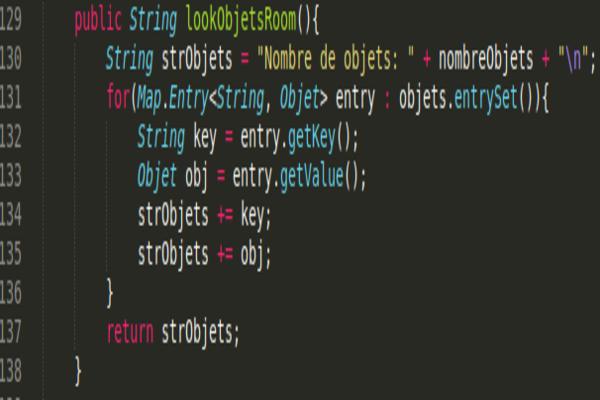
\includegraphics[scale=0.3]{captures/it2_8.png}
\end{center}

\subsection{\textcolor{bb}{Exercice 7.22.1 :}}
Optionnel.

\subsection{\textcolor{bb}{Exercice 7.22.2 :}}
Intégration des objets faites.

\subsection{\textcolor{bb}{Exercice 7.23, Exercice 7.24 et Exercice 7.25:}}
marche très bien.

\subsection{\textcolor{bb}{Exercice 7.26 :}}
\textbf{\textcolor{gg}{Apprentissage: Stack, push(), pop(), empty(), peek() :}\\
\textcolor{bb}{\href{https://docs.oracle.com/javase/8/docs/api/java/util/Stack.html}{https://docs.oracle.com/javase/8/docs/api/java/util/Stack.html}}}
\begin{center}
\begin{tabular}{|l|l|}
\hline
boolean & empty() \\ & Teste si cette pile est vide. \\
\hline
E & peek()\\ & Regarde l'objet en haut de cette pile sans le retirer de la pile.\\
\hline
E &pop()\\ & Supprime l'objet en haut de cette pile et renvoie cet objet en\\ &  tant que valeur de cette fonction.\\
\hline
E & push(E item)\\ & Pousse un objet sur le dessus de cette pile.\\
\hline
int & search(Object o)\\ & Retourne la position basée sur 1 où un objet est sur cette pile.\\
\hline
\end{tabular}
\end{center}

\subsection{\textcolor{bb}{Exercice 7.26.1 :}}
Génération des 2 javadoc du projet en utilisant :\\
javadoc -d docprog -author -version -private -linksource *.java\\
javadoc -d docuser -author -version *.java


\section{\textcolor{rr}{Itération 3 :}}
\subsection{\textcolor{bb}{Exercice7.28.1 :}}
Création de la commande test acceptant un second mot qui représente un nom de fichier, et exécute toutes les commandes lues dans ce fichier texte, les classes à modifier  sont "CommandWord" et "GameEngine" :
\begin{center}
	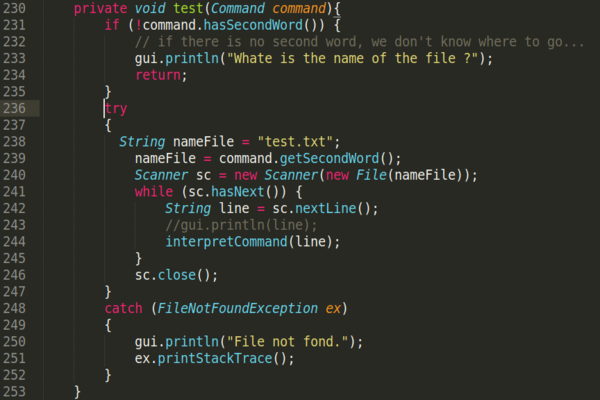
\includegraphics[scale=0.4]{captures/it3_1.png}
\end{center}
\textbf{\textcolor{gg}{Apprentissage lecture de fichiers de text, hasNext(), next(), exceptions :}} Fait.\\
\textbf{\textcolor{bb}{\href{https://docs.oracle.com/javase/8/docs/api/java/util/Scanner.html}{https://docs.oracle.com/javase/8/docs/api/java/util/Scanner.html}}}\\
\textbf{\textcolor{bb}{\href{https://docs.oracle.com/javase/8/docs/api/java/io/File.html}{https://docs.oracle.com/javase/8/docs/api/java/io/File.html}}}

\subsection{\textcolor{bb}{Exercice 7.28.2:}}
Exercice fait par rapport au scénario développé dans ce jeu.

\subsection{\textcolor{bb}{Exercice 7.29:}}
L’ajout de la classe Player  qui contient un nom, le poid maximum qu’il supporte, le poid qu’il porte actuellement, un gain et les objets que le joueur a  ramassé ou mangé.
\begin{center}
	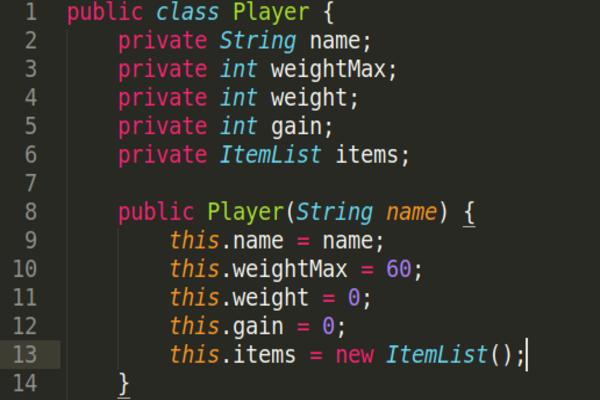
\includegraphics[scale=0.4]{captures/it3_2.png}
\end{center}

\subsection{\textcolor{bb}{Exercice 7.30:}}
L’ajout de deux commandes take et drop qui s’occupe de la  prise ou du dépôt d’un objet  déjà prit  respectivement, les classes modifiées  sont "CommandWord" et "GameEngine":
\begin{center}
	\begin{minipage}{0.4 \textwidth}
		\begin{flushleft}
			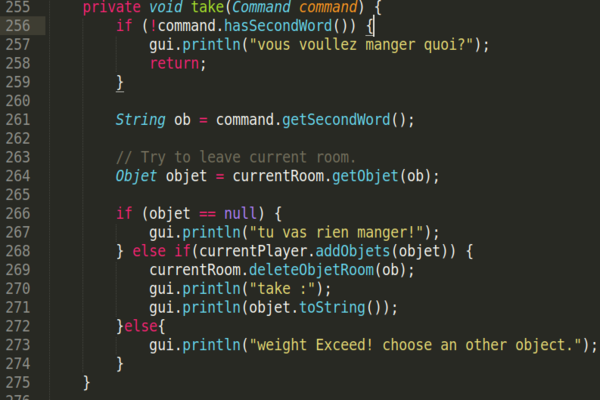
\includegraphics[scale=0.23]{captures/it3_3.png}
		\end{flushleft}
	\end{minipage}
	\begin{minipage}{0.4 \textwidth}
		\begin{flushright}
			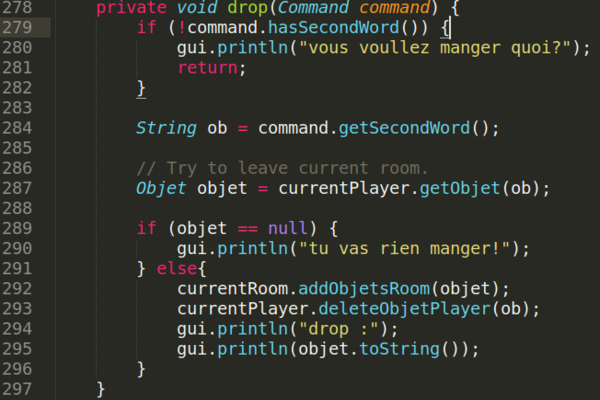
\includegraphics[scale=0.23]{captures/it3_4.png}
		\end{flushright}
	\end{minipage}
\end{center}

\subsection{\textcolor{bb}{Exercice 7.31 \& exercice 7.31.1:}}
Porter items  est fait.\\
Création de la classe ItemList qui gère une liste d'items et  mutualiser la gestion des items qui ont  été dupliqué dans Room et dans Player.
\begin{center}
	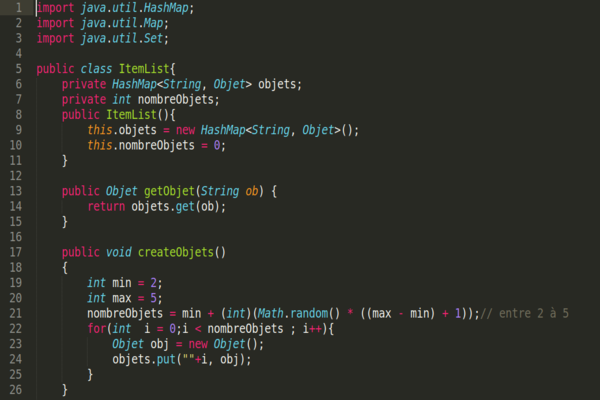
\includegraphics[scale=0.4]{captures/it3_5.png}
\end{center}
\begin{center}
	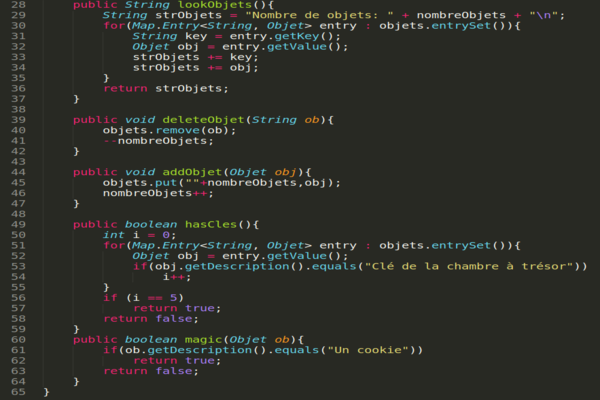
\includegraphics[scale=0.4]{captures/it3_6.png}
\end{center}
\subsection{\textcolor{bb}{Exercice 7.32 \& exercice 7.33 :}}

Poid max et inventaire c’est fait dans  dans la classe Player et  GameEngine avec une nouvelle commande items.
\begin{center}
	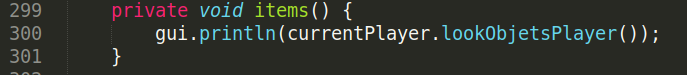
\includegraphics[scale=0.4]{captures/it3_7.png}
\end{center}
\begin{center}
	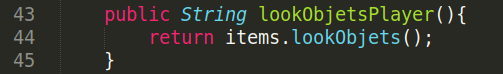
\includegraphics[scale=0.4]{captures/it3_8.png}
\end{center}
Et cette dernière appelle la méthode lookObjets dans la classe ItemsList.


\subsection{\textcolor{bb}{Exercice 7.34:}}
L’ajout d’un objet magic cookie qui augmente le poid maximum d’un joueur, qui appelle la méthode magic  de la classe ItemsList.
\begin{center}
	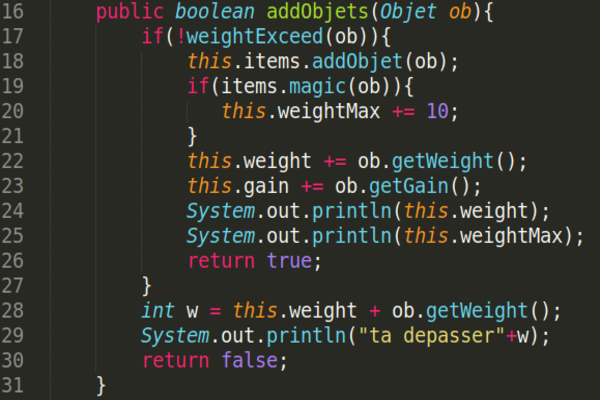
\includegraphics[scale=0.4]{captures/it3_9.png}
\end{center}
\textbf{\textcolor{gg}{Apprentisage de enum et values : fait.}}\\
\textbf{\textcolor{bb}{\href{https://docs.oracle.com/javase/8/docs/api/java/lang/Enum.html}{https://docs.oracle.com/javase/8/docs/api/java/lang/Enum.html}}}

\subsection{\textcolor{bb}{Exercice 7.35 \& exercice 7.35.1:}}
Consultation du code source du projet zuul-with-enums-v1 pour voir comment  le type CommandWord est utilisé. Les classes Command, CommandWords, Game et Parser sont toutes  adaptées dans cette version de notre projet, pour prendre en charge ce changement. le programme fonctionne toujours comme prévu.

\subsection{\textcolor{bb}{Exercice 7.35.2:}}
En s'inspirant de processCommand() de la classe Game dans zuul-withenums-v1, on a remplacé dans interpreteCommand() de la classe GameEngine la suite de if else par un switch (autorisé sur un type énuméré !) .
\begin{center}
	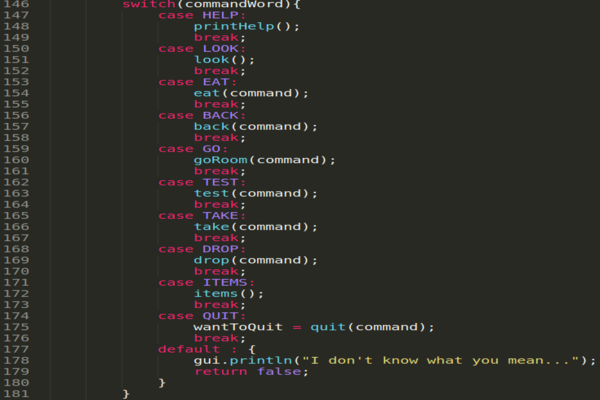
\includegraphics[scale=0.4]{captures/it3_10.png}
\end{center}

\subsection{\textcolor{bb}{Exercice 7.36, exercice 7.37, exercice 7.38, exercice 7.39, exercice 7.40 et exercice 7.41:}}
Déjà fait.



\section{\textcolor{rr}{Itération 4 :}}
\subsection{\textcolor{bb}{Exercice7.42  \& exercice7.42.1 :}}
Temps limite implémenter, on comptant le nombre de commande tapez au clavier dans un premier temps, après on à utiliser le temps réel pour implanter la limite demandée, dans la classe GameEngine:
\begin{center}
	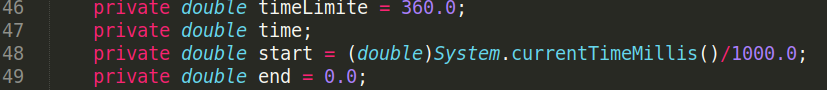
\includegraphics[scale=0.35]{captures/it4_1.png}
\end{center}

\subsection{\textcolor{bb}{Exercice7.43 :}}
Une trap door n'est pas une trap room. La pièce concernée peut très bien avoir plusieurs sorties, mais l'une d'entre-elles ne doit être franchissable que dans un seul sens.\\
On a implémenter la trap room de la manier suivant : on a définit des sortis pour une room mais dans la room d’après on définit la room précédente.

\subsection{\textcolor{bb}{Exercice7.44 :}}
l’implémentation du Beamer :
Le téléporteur (beamer) doit pouvoir être ramassé dans une première pièce, peut ensuite être chargé dans une deuxième pièce, puis déclenché dans une troisième ; il peut éventuellement être réutilisable, mais dans ce cas, il doit obligatoirement être rechargé, les classes modifier sont : GameEngine, Objet et  WordCommand.
\begin{center}
	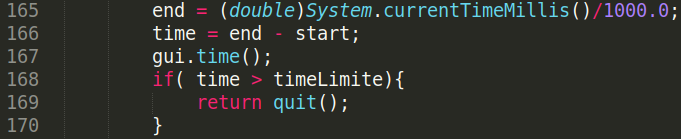
\includegraphics[scale=0.3]{captures/it4_2.png}
\end{center}
\begin{center}
	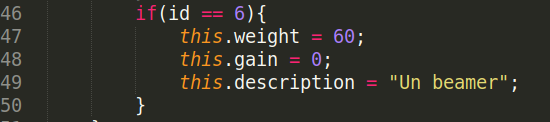
\includegraphics[scale=0.4]{captures/it4_3.png}
\end{center}
Pour ça j’ai du surcharger la méthode goRoom :
\begin{center}
	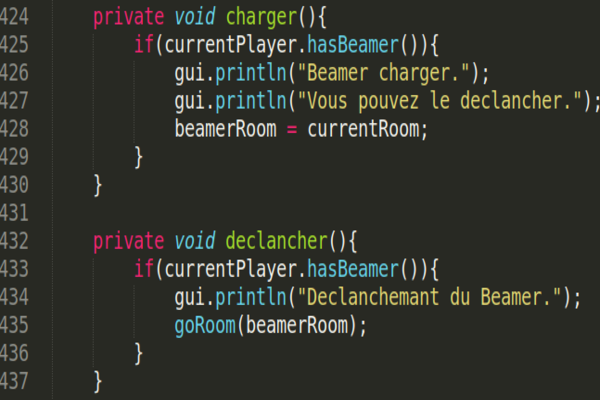
\includegraphics[scale=0.4]{captures/it4_4.png}
\end{center}

\subsection{\textcolor{bb}{Exercice7.45 \& exercice7.45.1 :}}
\textbf{\textcolor{gg}{Apprentissage : Random, nextInt(), seed:}\\ 
\textcolor{bb}{\href{https://docs.oracle.com/javase/8/docs/api/java/util/Random.html}{https://docs.oracle.com/javase/8/docs/api/java/util/Random.html}}}

\subsection{\textcolor{bb}{Exercice7.46 :}}
Pour implémente transporter room on a ajouter une méthode getRandomRoom :
\begin{center}
	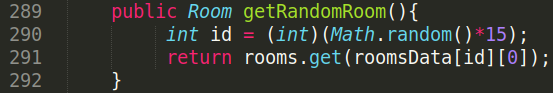
\includegraphics[scale=0.5]{captures/it4_5.png}
\end{center}
Dans la méthode goRoomon dans  la classe GameEngine on ajouter ces lignes :
\begin{center}
	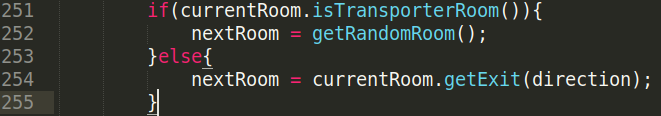
\includegraphics[scale=0.4]{captures/it4_6.png}
\end{center}
Dans la classe Room on a ajouté : 
\begin{center}
	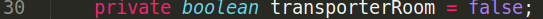
\includegraphics[scale=0.5]{captures/it4_7.png}
\end{center}
\begin{center}
	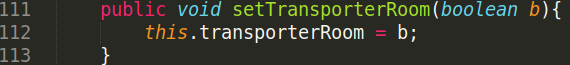
\includegraphics[scale=0.49]{captures/it4_8.png}
\end{center}

\subsection{\textcolor{bb}{Exercice7.46.2 :}}

\subsection{\textcolor{bb}{Exercice7.46.3 :}}
Les commentaire sont ajouter à tous les classes et la javadoc et générer.


\subsection{\textcolor{bb}{Exercice7.47:}}
Abstract Command.\\
\textbf{\textcolor{gg}{Apprentissage : polymorphisme}\\
\textcolor{bb}{\href{https://docs.oracle.com/javase/tutorial/java/IandI/polymorphism.html}{https://docs.oracle.com/javase/tutorial/java/IandI/polymorphism.html}}}

\subsection{\textcolor{bb}{Exercice7.47.1:}}
Découpage du projet en paquetage :
\begin{itemize}
\item \textbf{Game.java}.
\item \textbf{pkg\_command :} Command.java, CommandWord.java, CommandWords.java et Parser.java. 
\item \textbf{pkg\_interface :} GameEngine.java et UserInterface.java.
\item \textbf{pkg\_objets :} ItemList.java, Objet.java, Player.java et Room.java.
\end{itemize}
\textbf{\textcolor{gg}{Apprentissage : paquetage anonyme/par défaut.}\\
\textcolor{bb}{\href{https://docs.oracle.com/javase/tutorial/java/package/packages.html}{https://docs.oracle.com/javase/tutorial/java/package/packages.html}}} 

\subsection{\textcolor{bb}{Exercice 7.53: \& exercice 7.54 :}}
Dans la classe Game on a ajoute une méthode static main :
\begin{center}
	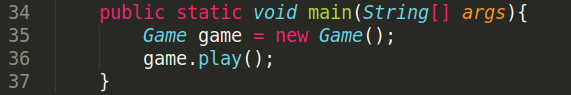
\includegraphics[scale=0.5]{captures/it4_9.png}
\end{center}

\subsection{\textcolor{bb}{Exercice 7.58:}}
Fabrication du fichier .jar :
\begin{itemize}
\item Dans le dossier zuul-v4 :\\
\textbf{javac -d "./classes/" ./src/Game.java}
\item Dans le dossier classes :\\
\textbf{jar cvfm ../zuul-v4.jar MANIFEST.MF  . ../images/}
\item Dans le dossier zuul-v4:\\
\textbf{java -jar zuul-v4.jar}
\end{itemize}

\subsection{\textcolor{bb}{Exercice 7.59:}}
Sauvegarde de l’état du jeu (en Java) ; la commande acceptera un nom de fichier en second mot. Deux solutions possibles :
\begin{enumerate}
\item Sauvegarder les éléments du jeu.
\item Sauvegarder les commandes exécutées.	
\end{enumerate}
On a opté pour la première solutions avec la sérialisation des données, ou chaque classes que on veut sauvegarder empilements  l’interface Sérialisable.    
\begin{center}
	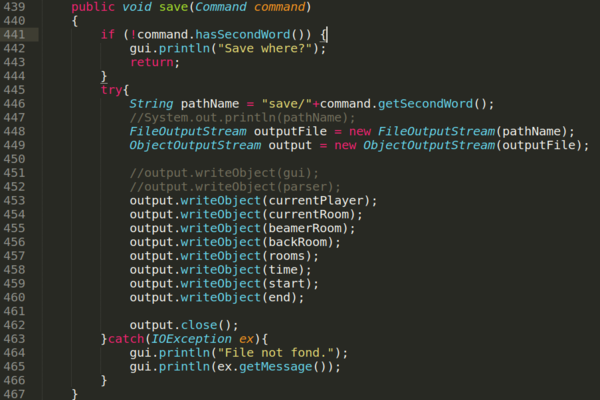
\includegraphics[scale=0.4]{captures/it4_10.png}
\end{center}
\begin{center}
	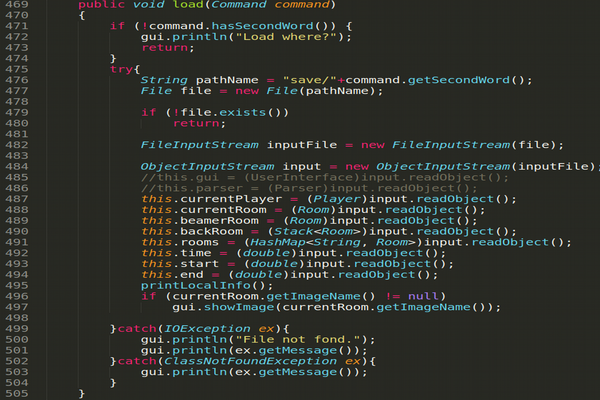
\includegraphics[scale=0.51]{captures/it4_11.png}
\end{center}



\chapter{Gestionnaire de stock}
\section{\textcolor{rr}{Itération 1}}
\subsection{\textcolor{bb}{Diagramme de cas d’utilisation }}
\begin{flushright}
 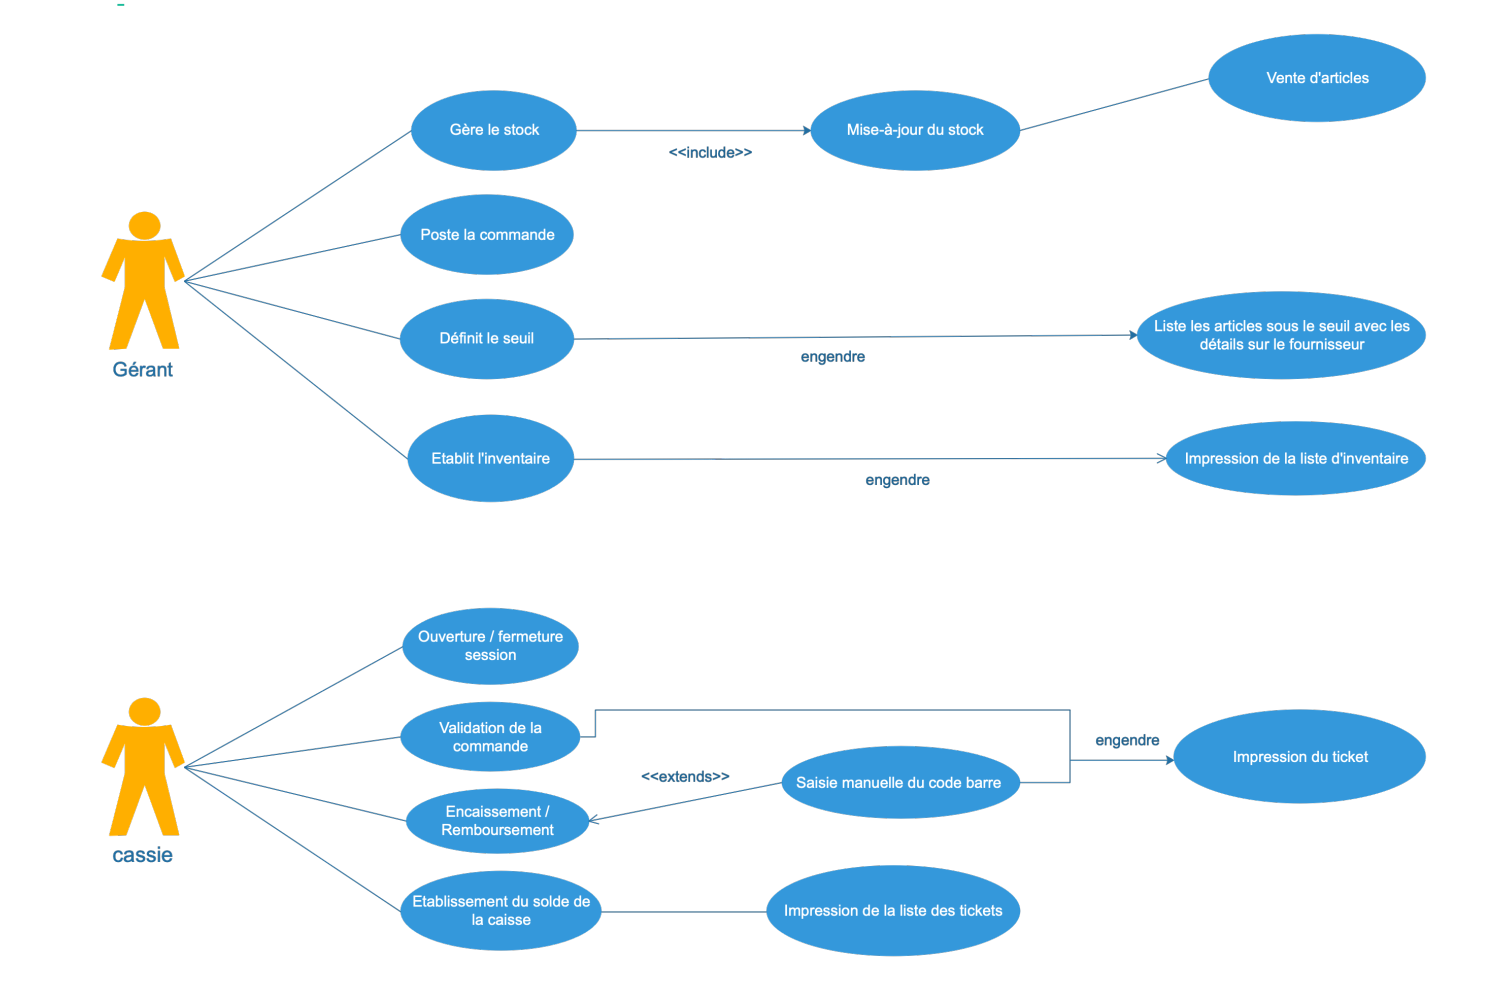
\includegraphics[scale=0.25]{captures/g_it1_1.png}
\end{flushright}


\subsection{\textcolor{bb}{Description des éléments}}
Le diagramme de cas d’utilisation modélisé ci dessous est représentation minimal des fonctionnalités de notre système de gestion de stock.\\
\textbf{Les acteurs :} 
\begin{itemize}
\item Le gérant.
\item Le caissier.
\end{itemize}
\textbf{Le système :}\\
En fait le système de gestion de stock est un ensemble de fonctionnalités qui collaborent entre elle modélisé d’une façon générique.\\
\textbf{Les fonctionnalités :}
\begin{itemize}
\item \textbf{Vente :} le détaillant grâce à la caisse peut vendre des produit scanné avec un scanner de code barre et cela va automatiquement diminuer le stock.
\item \textbf{ Passer une commande :} le détaillant grâce aux alertes de système peut savoir si la quantité d’un produit est passé au dessus de seuil fixé par le détaillant.
\item \textbf{Inventaire, liste fournisseur, définir le seuil :} le détaillant peut lister la totalité des articles en stock, voir la liste de ses fournisseur à la fois par article ou la totalité des fournisseur et il peut aussi mettre manuellement les seuils des articles pour être alerté grâce à ce dernier.
\end{itemize}

\subsection{\textcolor{bb}{ Le design des interfaces Homme-Machine de l’application}}


\section{\textcolor{rr}{Itération 2}}
\subsection{\textcolor{bb}{Étape 1 : Capture des exigences fonctionnelles}}
\subsubsection{Diagramme des cas d’utilisation}
\begin{center}
 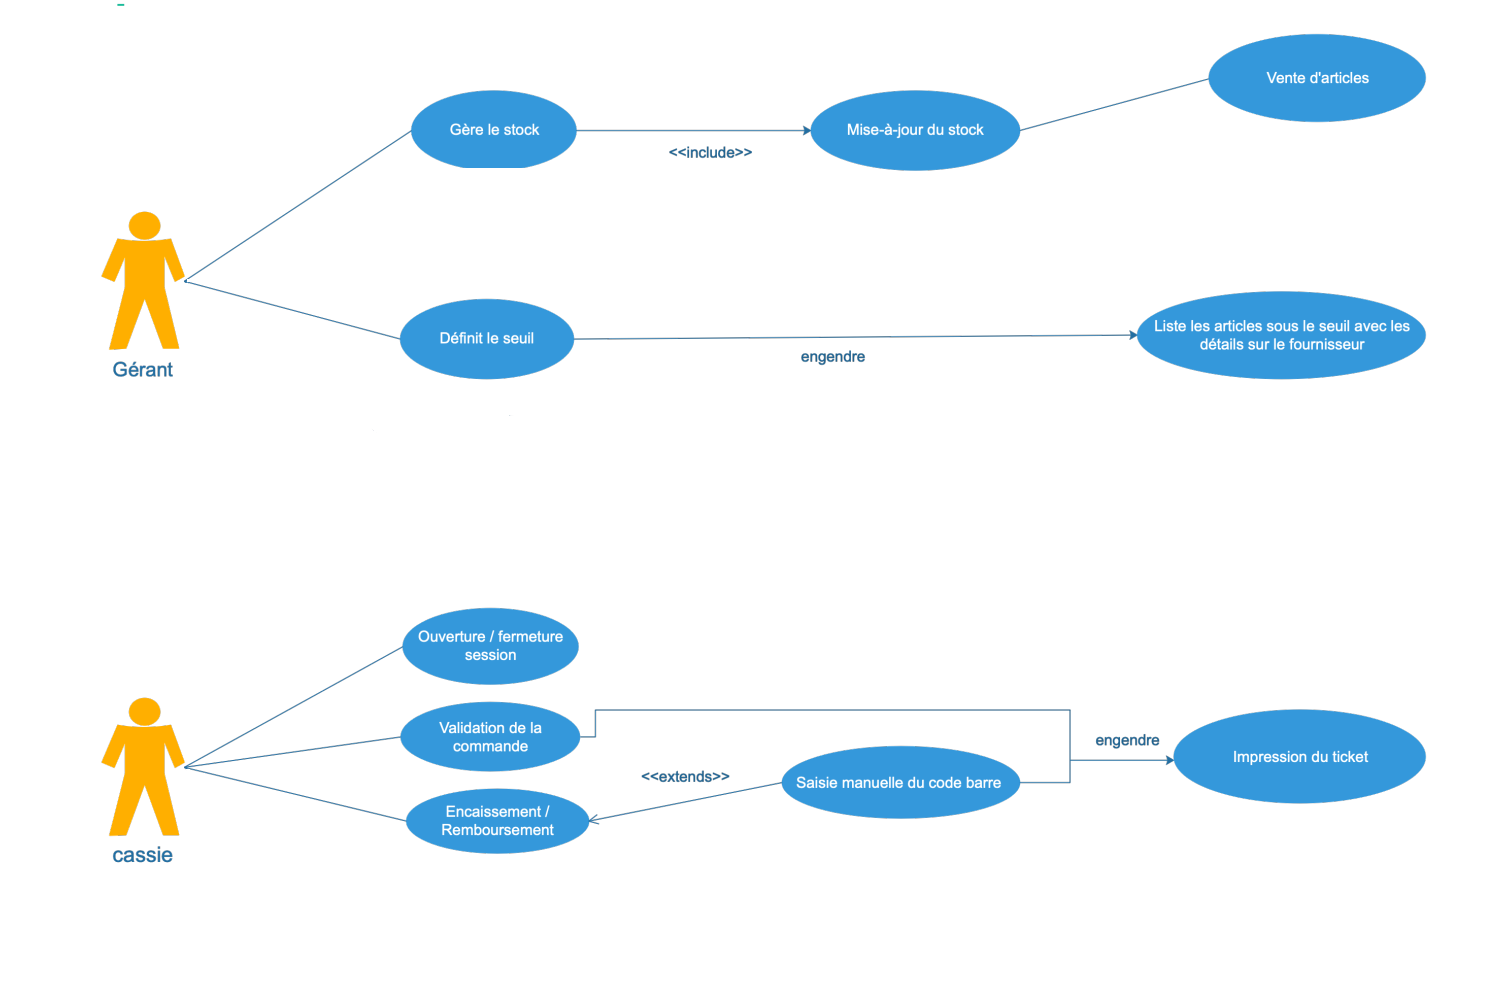
\includegraphics[scale=1]{captures/g_it1_2.png}
\end{center}

\subsubsection{Fiche descriptive des cas importants} 
\textbf{I- La caisse :}\\
Le système de la caisse contient une base de donnée concernant les articles, c’est-à-dire il contient toutes les informations de ces articles qui sont dans le stock ( nom, prix, quantité en stock…).\\
La caisse offre plusieurs fonctionnalités que le caissier utilise pour assurer la vente des produits, ce qui fait que ses cas d’utilisation sont importants.\\
\textbf{Acteurs :} le caissier.\\
Ci-dessous les étapes auxquelles le caissier est affronté  lors de son service:
\begin{itemize}
\item Ouverture / fermeture de la session : authentification du caissier.
\item Scanner les articles :
	\begin{itemize}
		\item  Si l’article est reconnu : la caisse émet un bip et affiche le nom et le prix de l’article.
		\item Sinon : le caissier doit saisir le code barre manuellement.
	\end{itemize}
\item Validation de la commande.
\item Le caissier appuie sur la touche <Total> s’il s’agit d’un achat, <Retour> s’il s’agit d’un remboursement.
\item Ouverture automatique du tiroir : elle est engendrée dans le cas d’un achat ou remboursement.
\item Règlement du total ou remboursement de la commande.
\item Fermeture automatique du tiroir.
\item Impression du ticket de caisse.
\item Mémoriser les articles scannées.
\item Impression de la liste des commandes effectuées.
\end{itemize}		
\textbf{Exception :} si le client effectue un retour, le caissier doit procéder au remboursement.\\[1cm]
\textbf{II- Le stock :} \\
\textbf{Acteurs :} le gérant.\\
Le système du stock contient exactement les mêmes informations qu’en caisse avec plus de détails sur les produits; le seuil de réassortiment . Pour une bonne gestion de stock , le gérant effectue plusieurs tâches :
\begin{itemize}
\item Visualiser les produits en stock.
\item Conserver les informations des articles.
\item Mémoriser les informations concernant les fournisseurs de chaque article (nom, numéro…).
\item Liste des articles sous le seuil avec les détails sur le fournisseur.
\item Mise-à-jour du stock.
\item Effectuer et imprimer l’inventaire.
\item Modifier les informations des détails concernant les articles.
\end{itemize}
\textbf{Exception :} si la quantité des articles est inférieure au seuil défini par le gérant, il doit lister tous les articles qui sont en dessous de ce seuil.
\subsection{\textcolor{bb}{Étape 2 : Étude du modèle statique}}
\subsubsection{Diagramme de classe :}
\begin{center}
 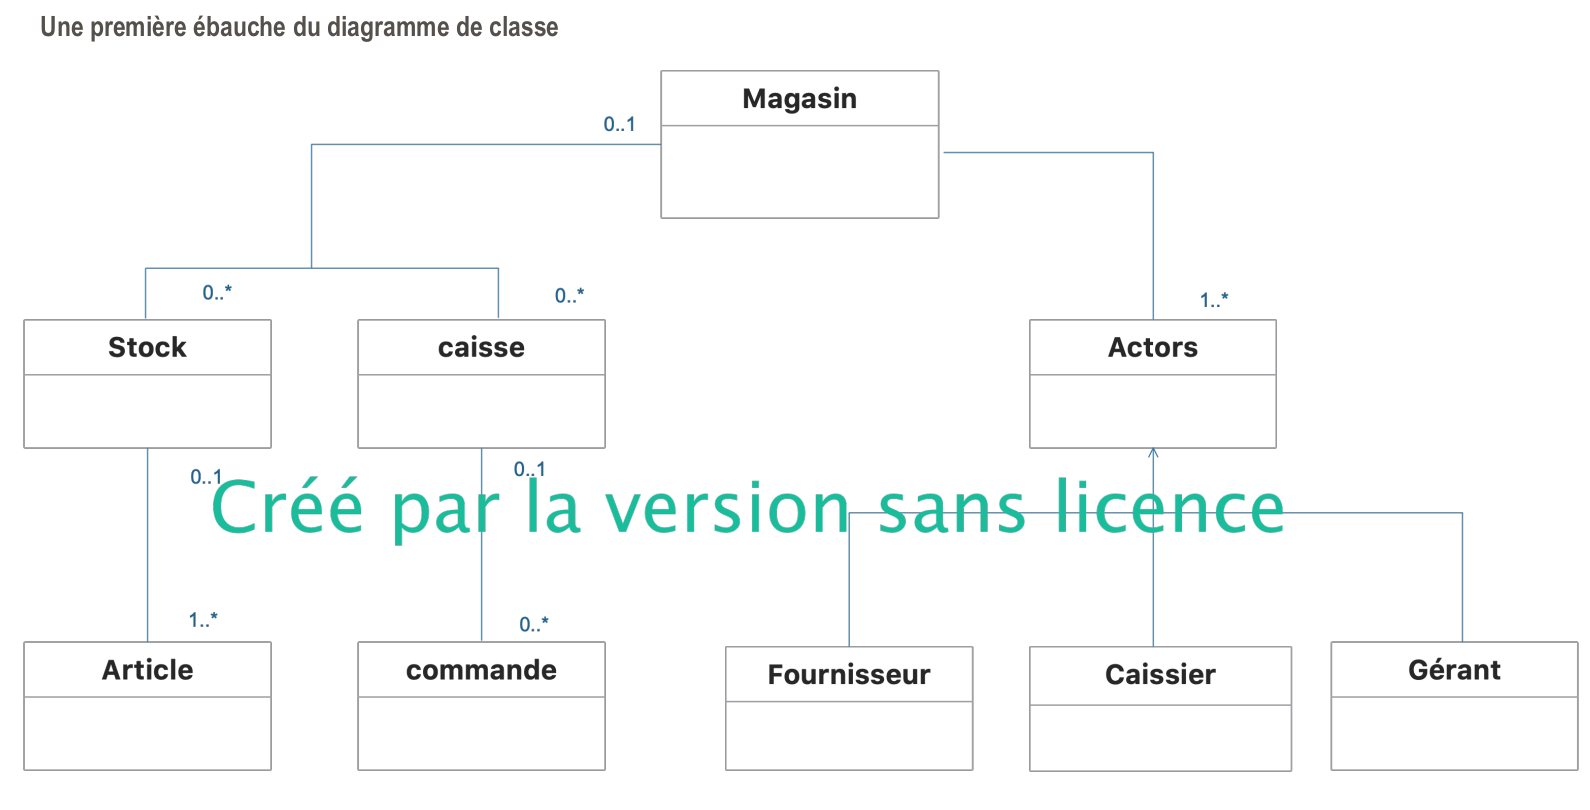
\includegraphics[scale=0.22]{captures/g_it2_1.png}
\end{center}

\subsubsection{Dictionnaire de données :}
Dans le diagramme de classe qu’on a établi, on a utilisé que les classes importantes.\\
Notre abstraction pour ce projet est la suivante :\\
On commence par la classe Magasin, c’est elle qui englobe toutes les classes, c’est-à-dire que dans un magasin on trouve 1 ou plusieurs employés, caisses, stock\\
Ensuite, au côté droit on trouve les personnes qui participent à ce système, donc on a une classe employés qui généralise les 3 classes suivantes : Fournisseur, Caissier et Gérant, car c’est les mêmes att25ributs qui se répètent dans ces dernières, c’est juste les fonctions de chacun qui diffèrent.\\
Au côté gauche, on trouve ce qui concerne les objets que les employés utilisent ou qu’on trouve dans le magasin, donc,  dans un magasin on peut trouver 1 ou plusieurs caisses et stocks.\\
Dans une caisse on peut valider plusieurs commandes comme on en peut en valider aucune.\\
Enfin, dans un stock on trouve tous les articles qui existent dans ce magasin.

\subsection{\textcolor{bb}{Étape 3 : Étude du modèle dynamique}}
\subsubsection{Diagramme de séquence pour le cas d’utilisation stock :}
\begin{center}
 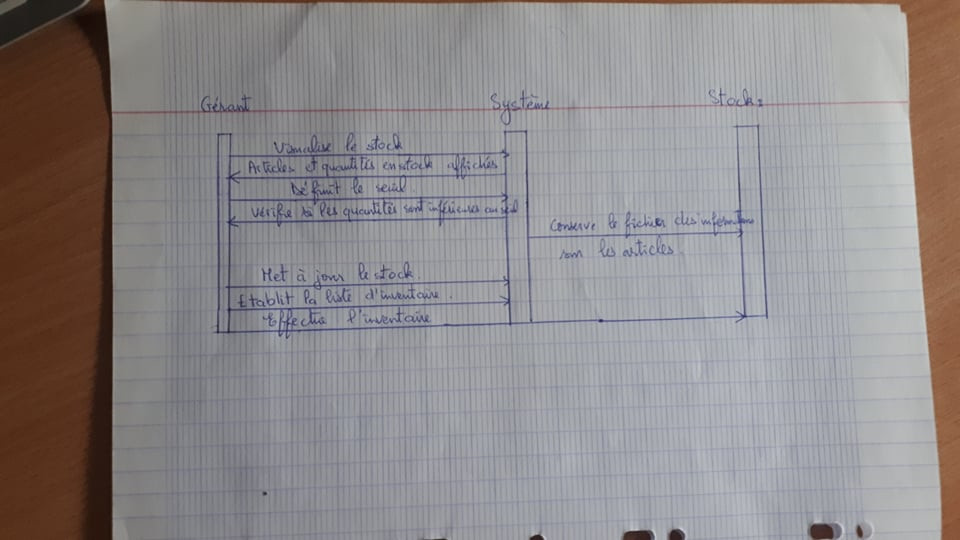
\includegraphics[scale=0.36]{captures/g_it2_2.jpg}
\end{center}

\subsubsection{Diagrammes de séquence pour le cas d’utilisation caisse avec respectivement l’achat et le remboursement :}
\begin{center}
 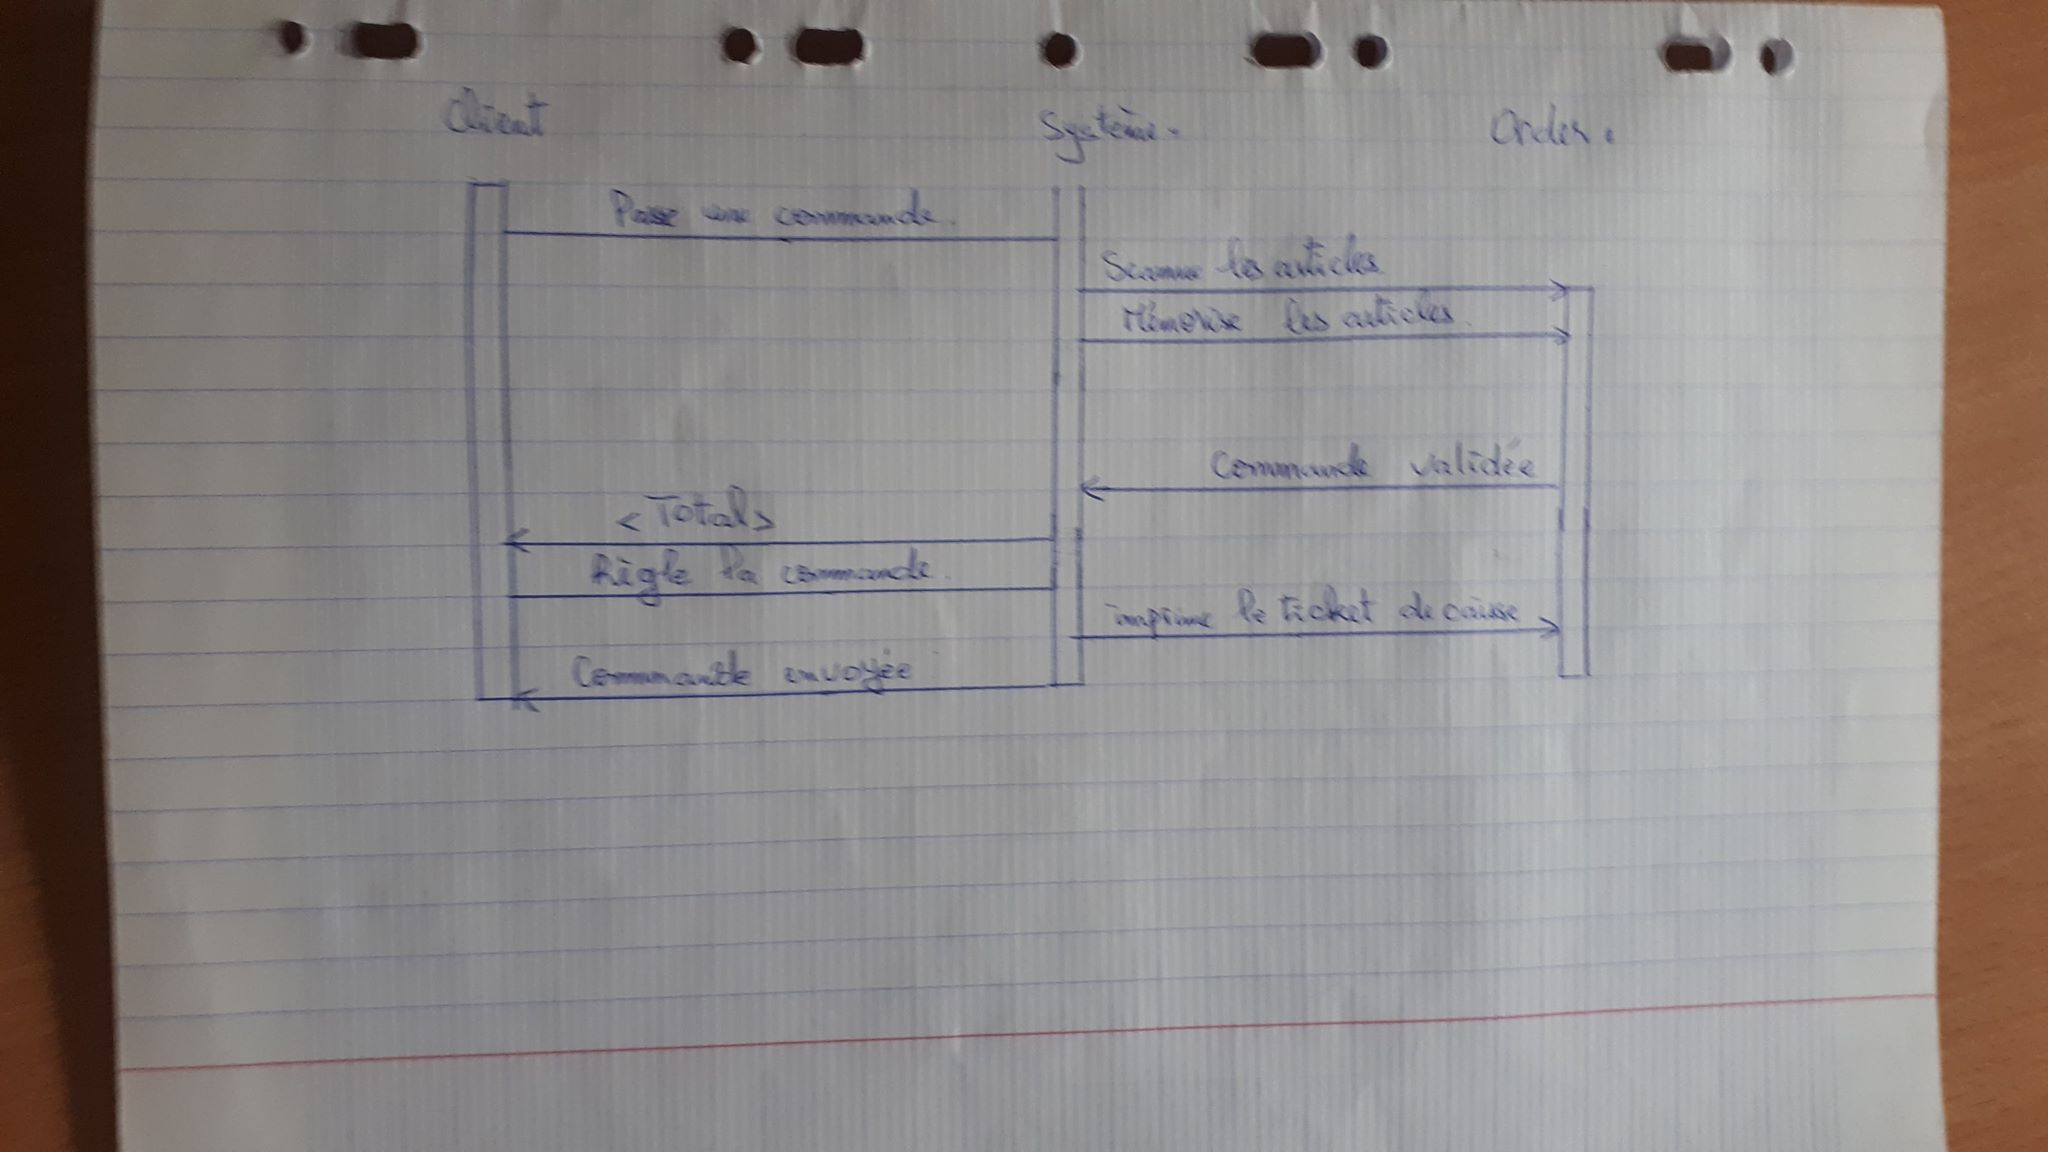
\includegraphics[scale=0.17]{captures/g_it2_3.jpg}
\end{center}
\begin{center}
 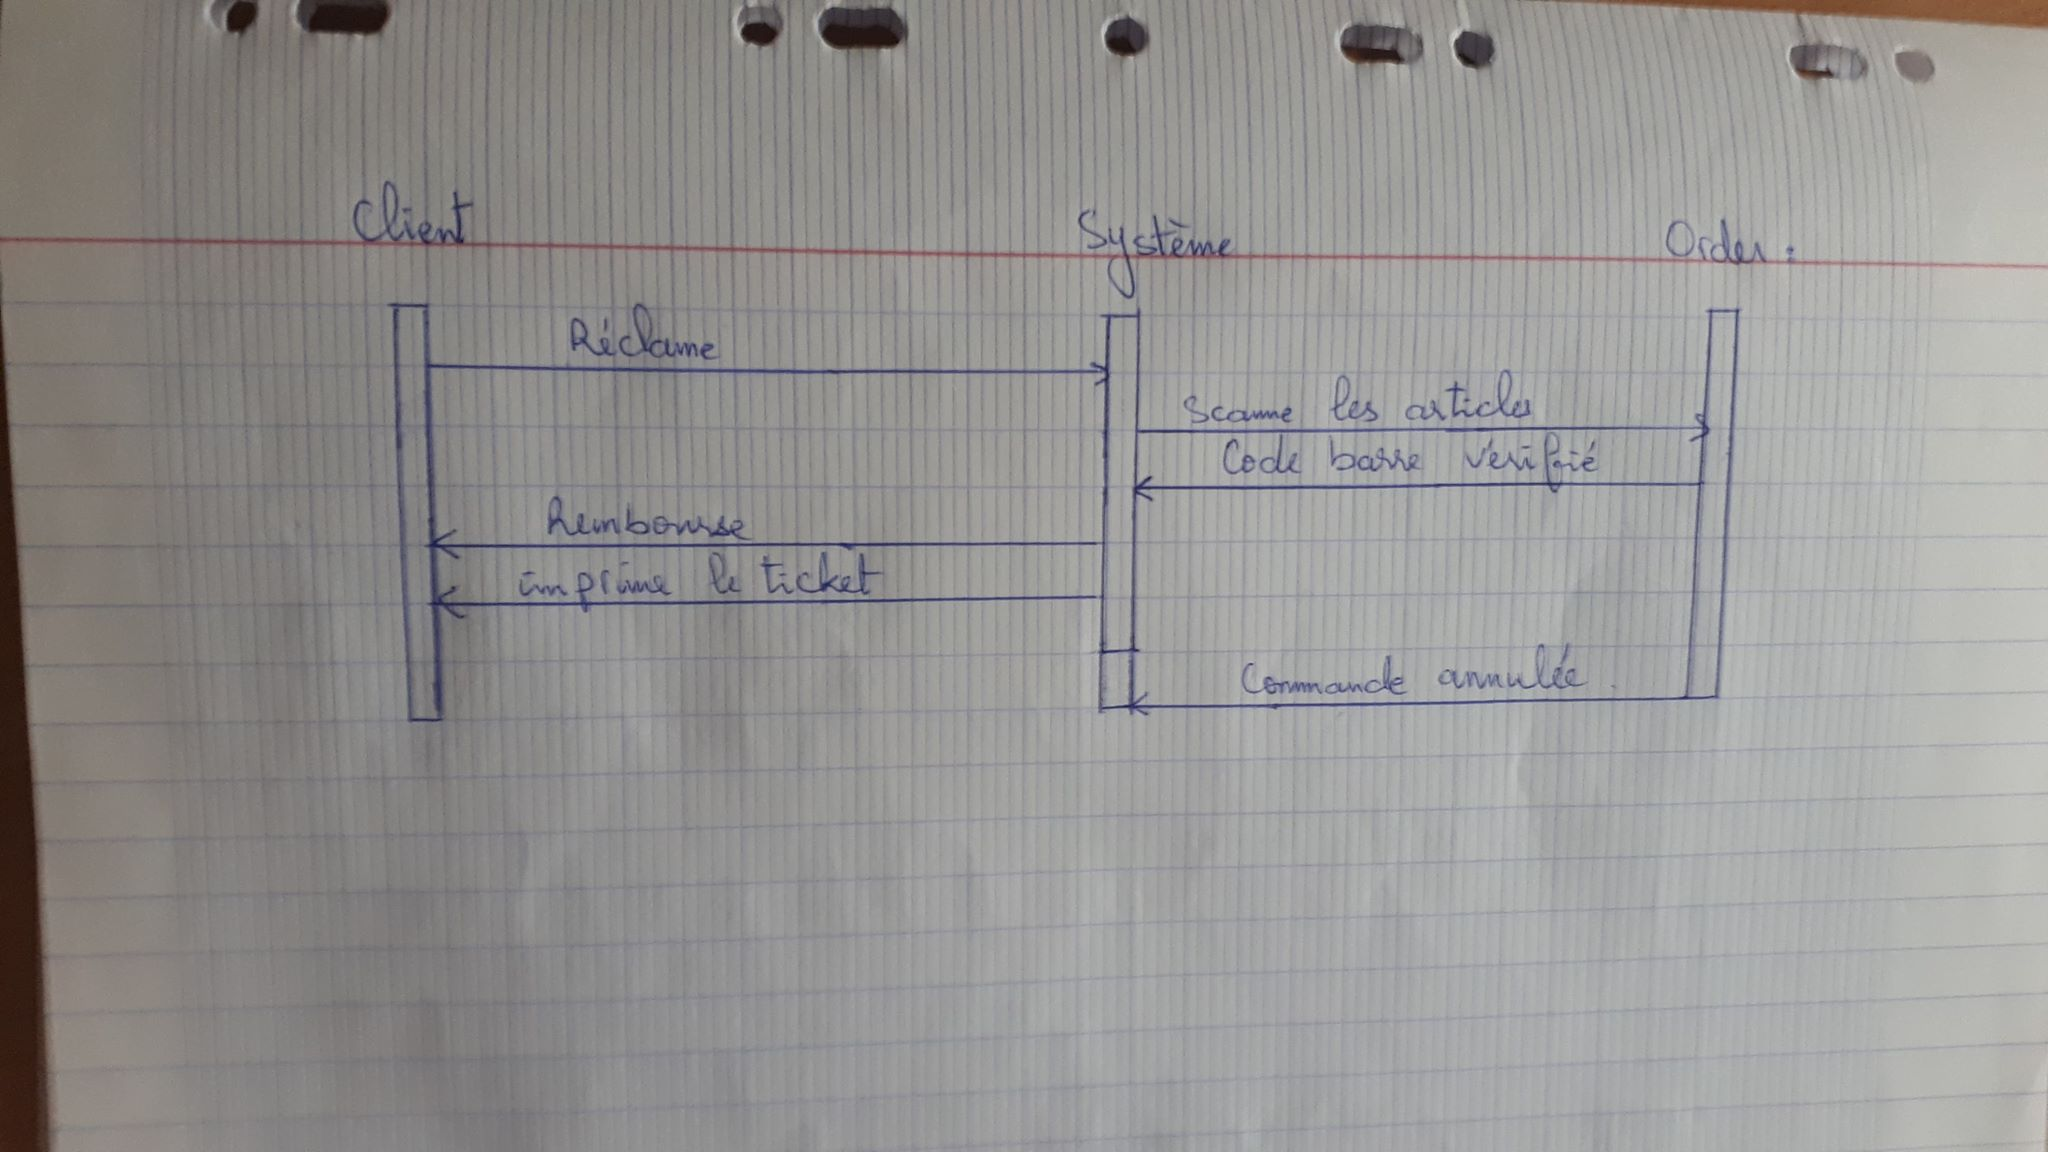
\includegraphics[scale=0.17]{captures/g_it2_4.jpg}
\end{center}

\section{\textcolor{rr}{Itération 3}}

\subsection{\textcolor{bb}{Phase de conception }}

Ci-dessous, les diagrammes de classe et de séquence techniques. En raison d’un problème d’installation de modelio, les diagrammes ont été effectués à la main.

\begin{center}
	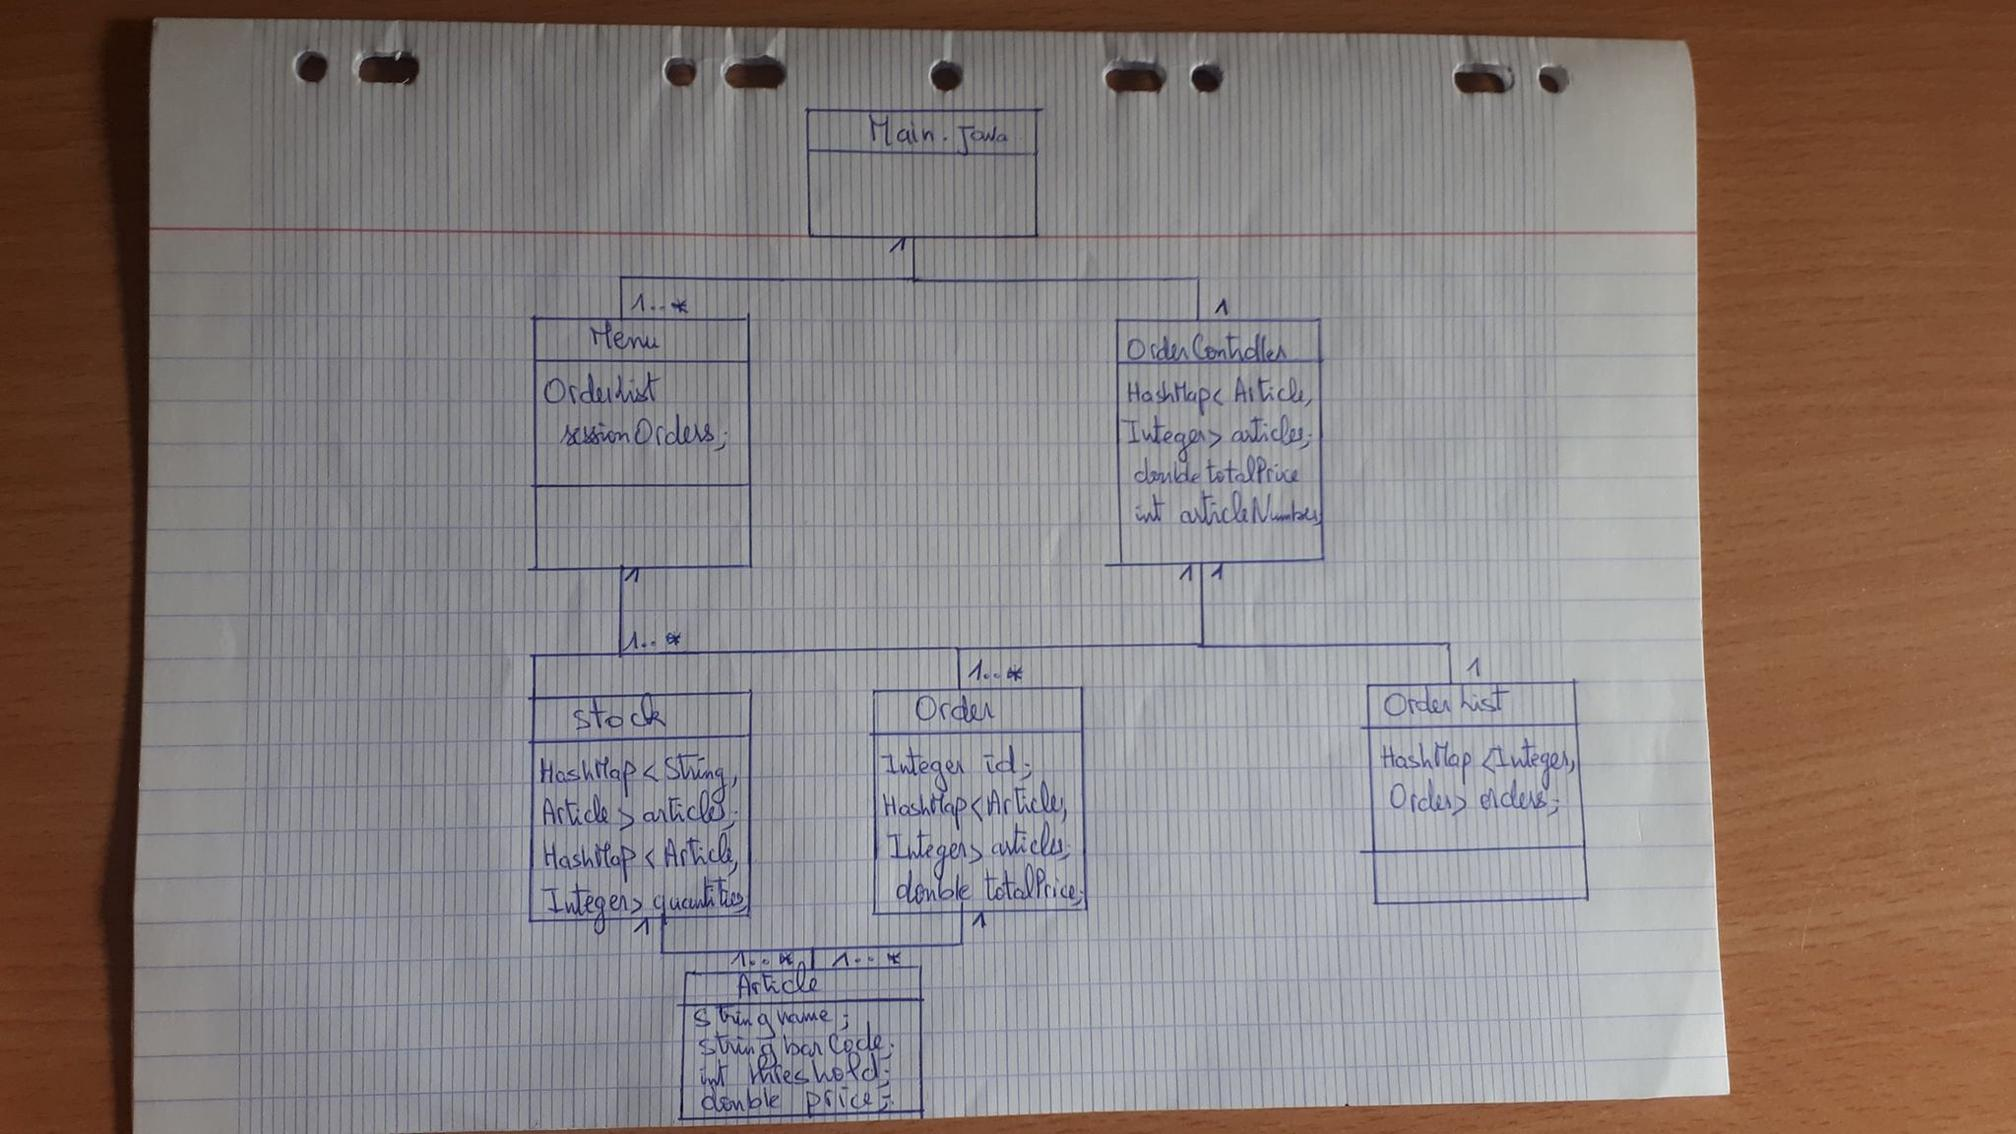
\includegraphics[scale=0.23]{captures/g_it3_1.jpg}
	\captionof{figure}{Ceci, représente le diagramme de classe technique.}
\end{center}	
\begin{center}
 	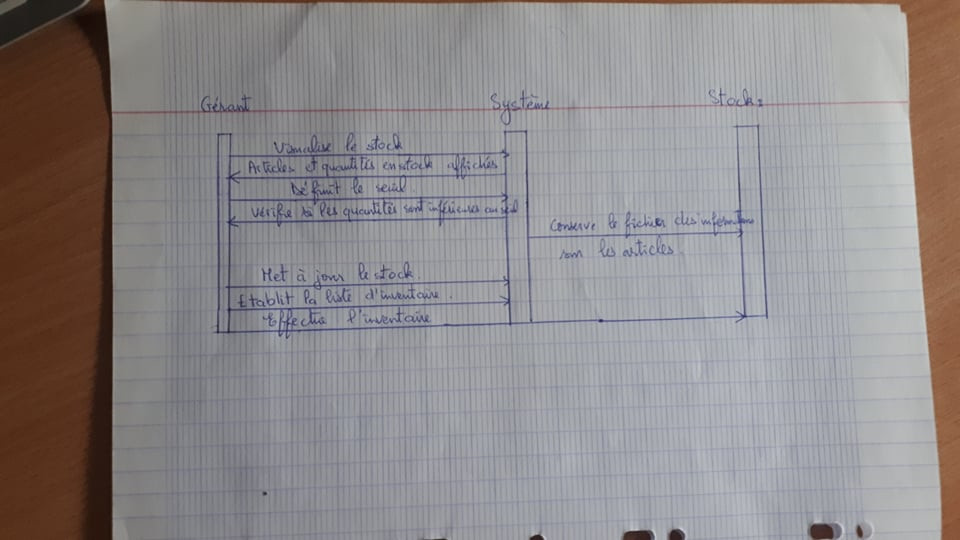
\includegraphics[scale=0.36]{captures/g_it3_2.jpg}
	\captionof{figure}{Ceci, représente le diagramme de séquence technique du stock.}
\end{center}	
\begin{center}
 	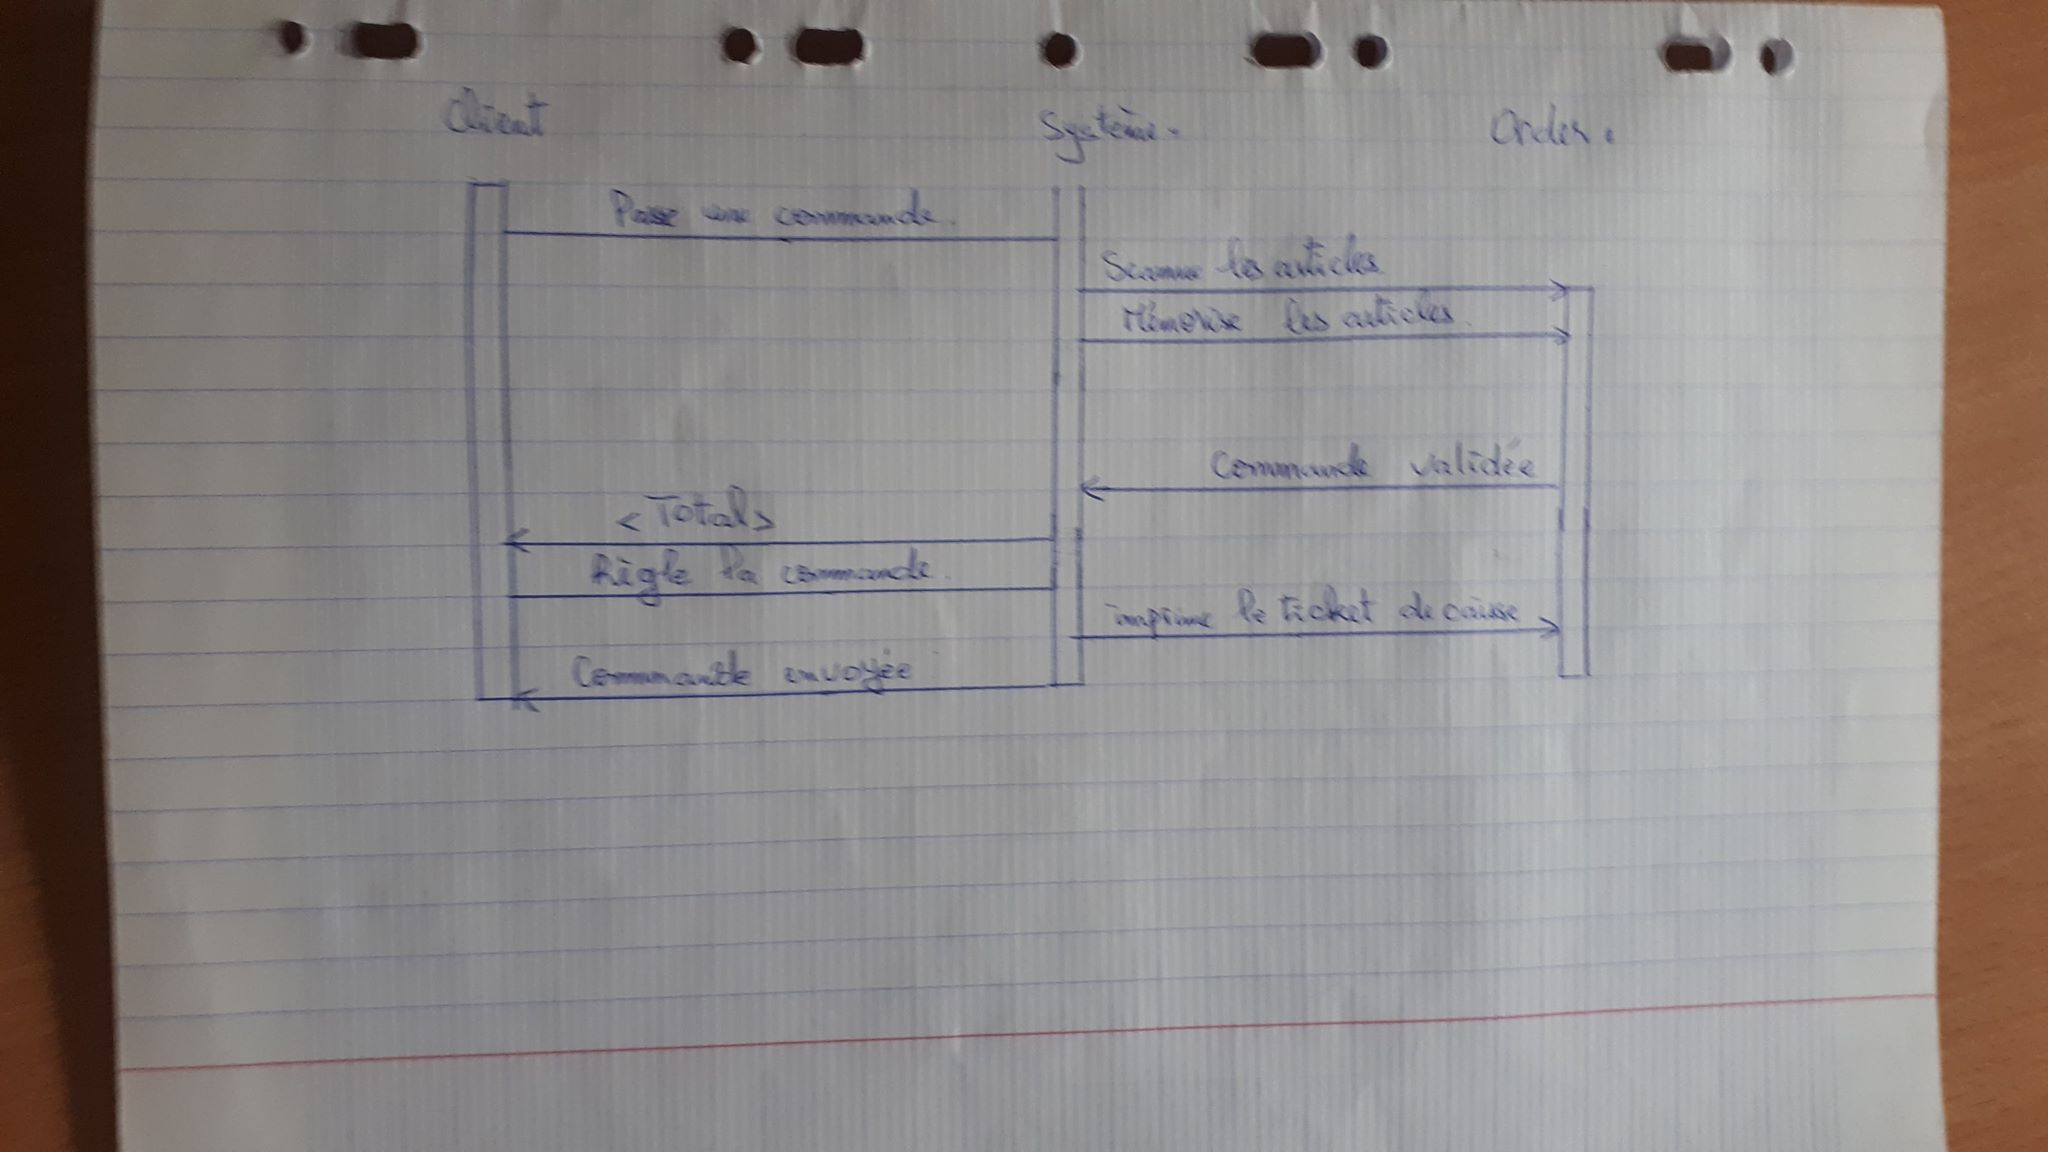
\includegraphics[scale=0.17]{captures/g_it3_3.jpg}
	\captionof{figure}{Ceci, représente le diagramme de séquence technique des commandes dans le cas d’un achat normal.}
\end{center}
\begin{center}
 	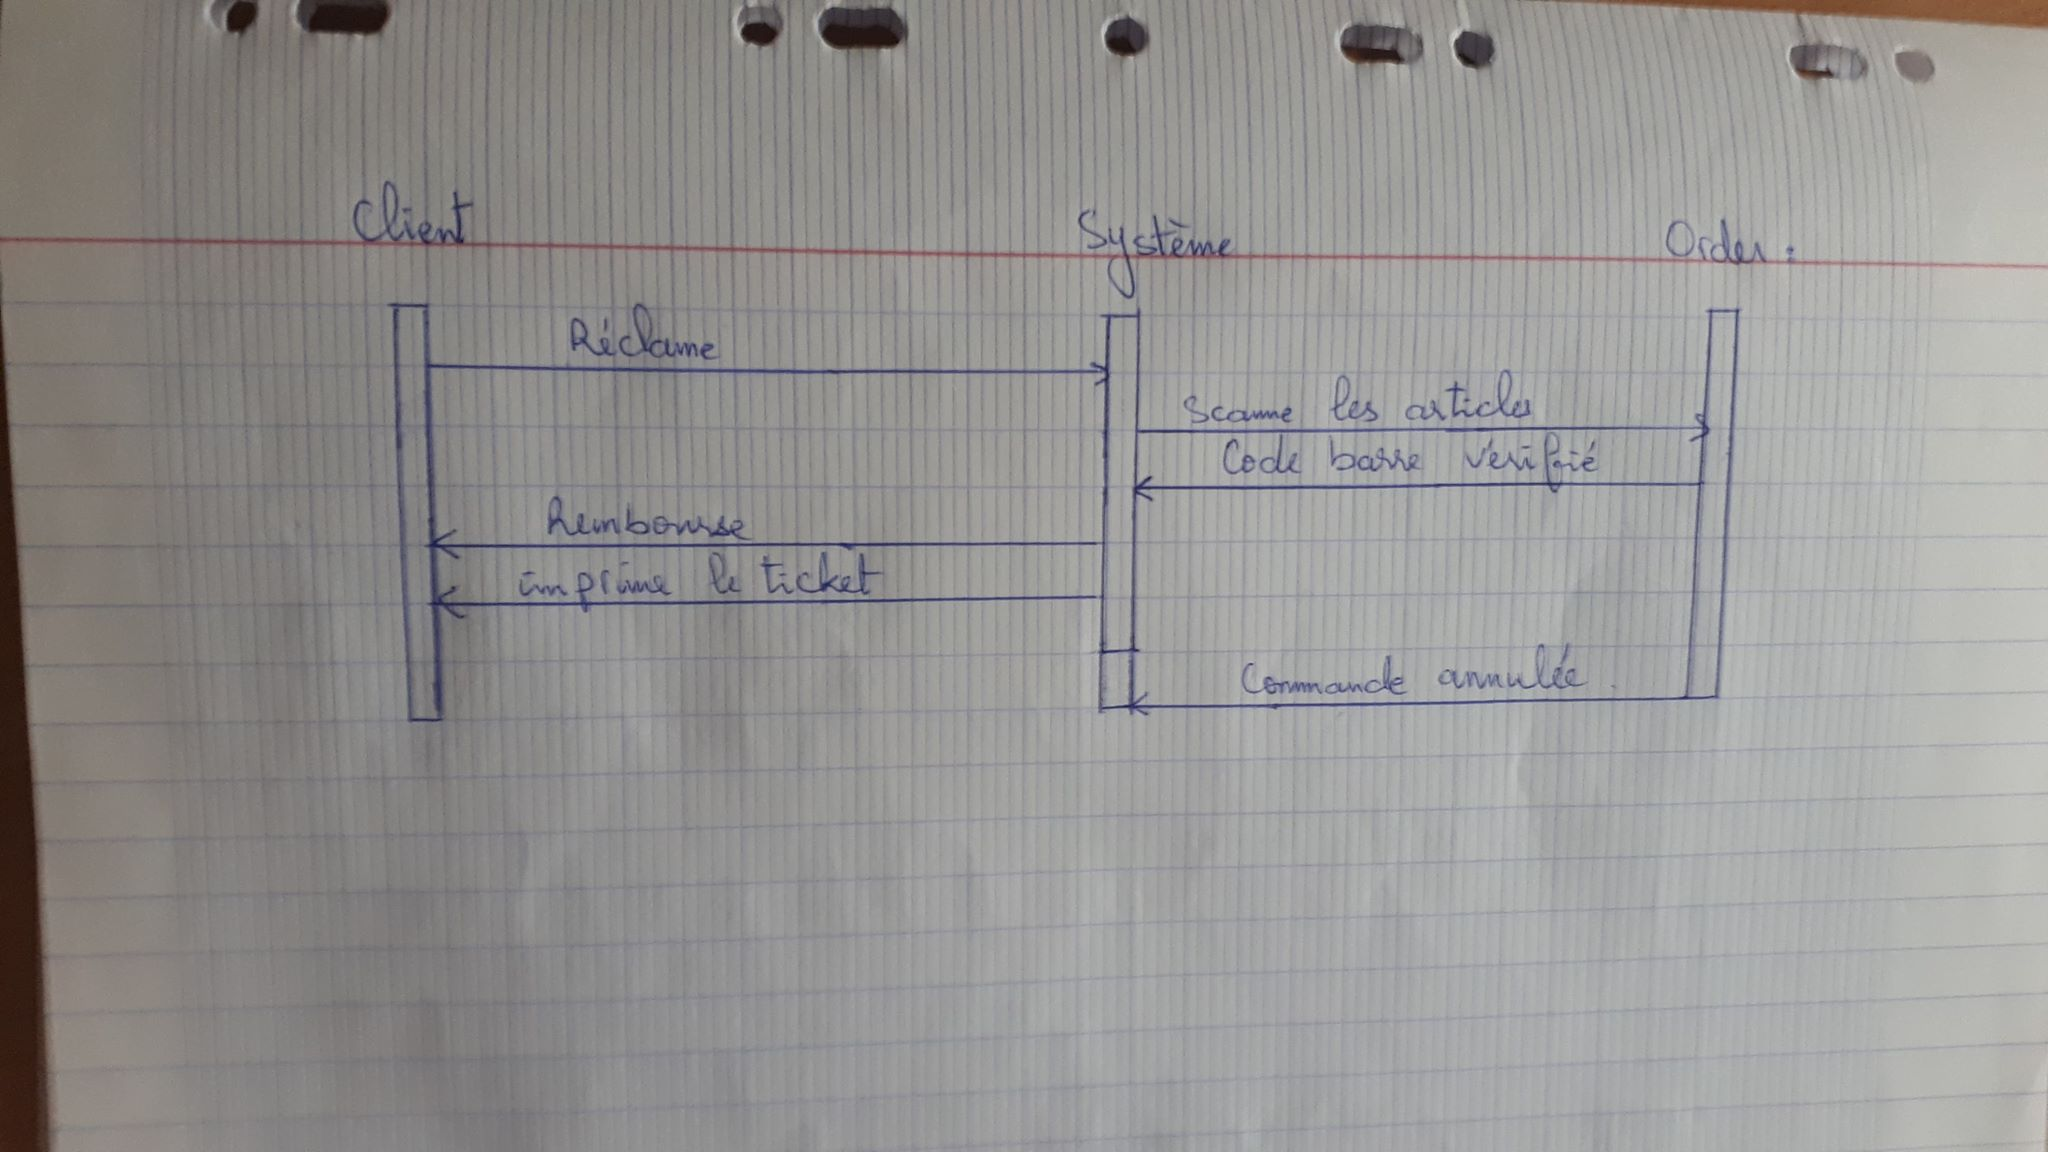
\includegraphics[scale=0.17]{captures/g_it3_4.jpg}
	\captionof{figure}{Ceci, représente le diagramme de séquence technique des commandes dans le cas d’un remboursement.}
\end{center}

\subsection{\textcolor{bb}{Phase d’implémentation}}
Pour commencer l’implémentation de l’application de gestion de stock, on devait établir des diagrammes des cas d’utilisation et séquences pour comprendre le fonctionnement de la gestion du stock c’est-à-dire comment passer une commande, comment mettre à jour le stock…
Ensuite, il fallait établir des diagrammes de classes, pour pouvoir démarrer l’implémentation c’est-à-dire définir les classes dont aura besoin pour créer cette application et ce qu’il y aura dans chaque classe.\\
Enfin, avant d’implémenter toutes ces classes, on a choisi l’architecture \textbf{\textcolor{gg}{MVC}}, avec :\\
\begin{itemize}
\item \textbf{Model :} les classes Article.java, Order.java, OrderList.java, Stock.java 
\item \textbf{View :}  la classe Menu.java ; c’est le menu de l’application.
\item \textbf{Controller :} OrderController.java ; c’est elle qui contrôle toutes les commandes.
\end{itemize}
\subsubsection{Compiler le programme dans le terminal :}

\textbf{I- Lancer la commande suivante dans le dossier bin :}\\
textcolor{rb}{javac -d "../bin" Main.java}\\
\textbf{II- Ensuite celle-ci :}\\
\textcolor{rb}{jar -cvfm Gestionnaire\_stock.jar MANIFEST.MF ./Model/*.class ./View/*.class ./Controller/*.class ./*.class}
\begin{center}
	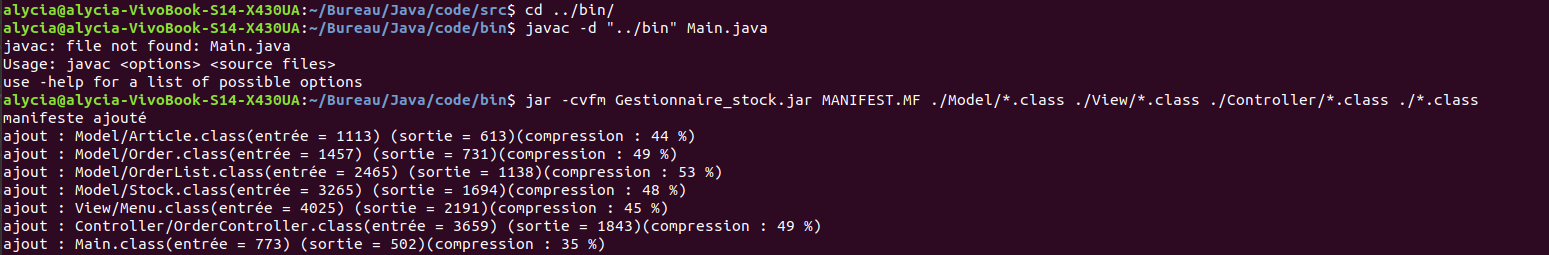
\includegraphics[scale=0.21]{captures/g_it3_5.png}
\end{center}
\textbf{III- Exécuter le programme avec la commande suivante :}\\
\textcolor{rb}{jar -cvfm Gestionnaire\_stock.jar MANIFEST.MF}
\begin{center}
	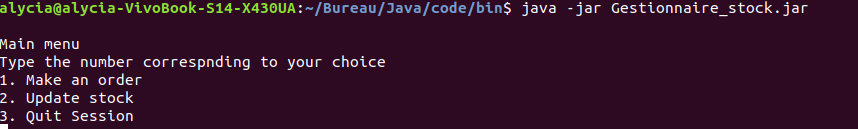
\includegraphics[scale=0.4]{captures/g_it3_6.png}
\end{center}
Le Menu principal de l’application se lance, pour effectuer une commande on sélectionne la première option, le Menu de celle-ci s’affiche :
\begin{center}
	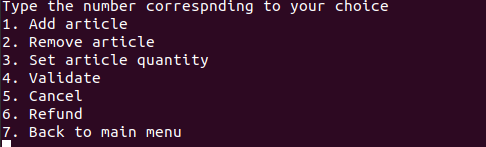
\includegraphics[scale=0.4]{captures/g_it3_7.png}
\end{center}

\paragraph{\textbf{Option 1 :}} ajouter un article:
On l’ajoute en insérant son code barre, si le code barre saisi est incorrect l’ajout de l’article ne s’effectuera pas.
\begin{center}
	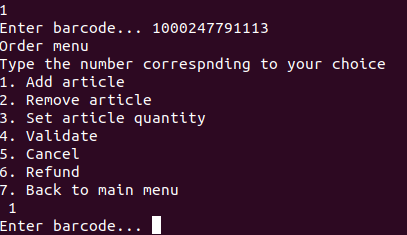
\includegraphics[scale=0.48]{captures/g_it3_8.png}
\end{center} 								

\paragraph{\textbf{Option 2 :}} Consiste à supprimer un article, en insérant son code barre :
\begin{center}
	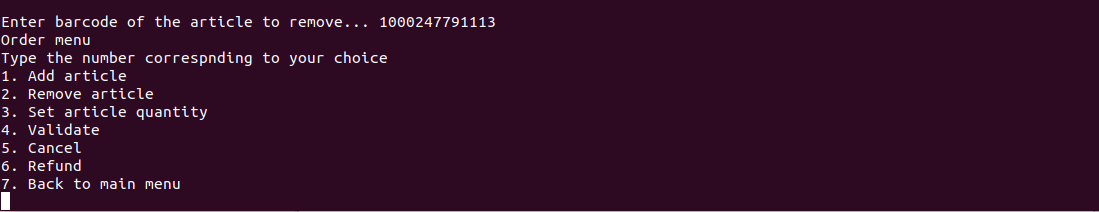
\includegraphics[scale=0.3]{captures/g_it3_9.png}
\end{center} 
\textbf{Option 3 :} Elle sert à modifier la quantité d’un article, en insérant son code barre et la nouvelle quantité.
\begin{center}
	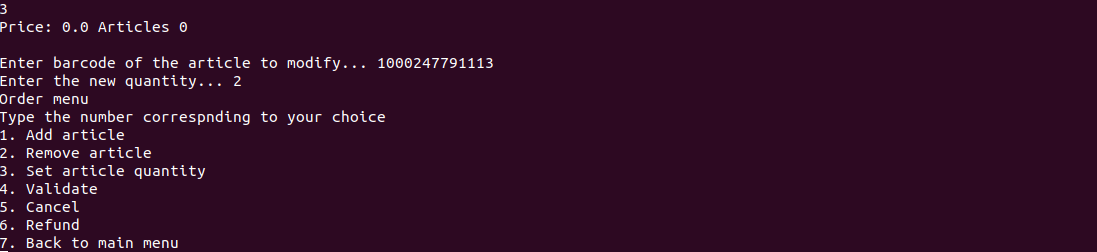
\includegraphics[scale=0.3]{captures/g_it3_10.png}
\end{center} 
\textbf{Option 4 :}  Elle sert à valider la commande.\\
\textbf{Option 5 :}  Consiste à annuler la commande courante et revenir au menu principal.\\
\textbf{Option 6 :}   Elle sert à rembourser le client, en insérant l’Id de la commande souhaitée.\\
\textbf{Option 7 :}  On revient au menu principal.\\[1cm]
Pour mettre à jour le stock, on choisit l’option 2 du menu principal, on aura donc le menu du stock :
\begin{center}
	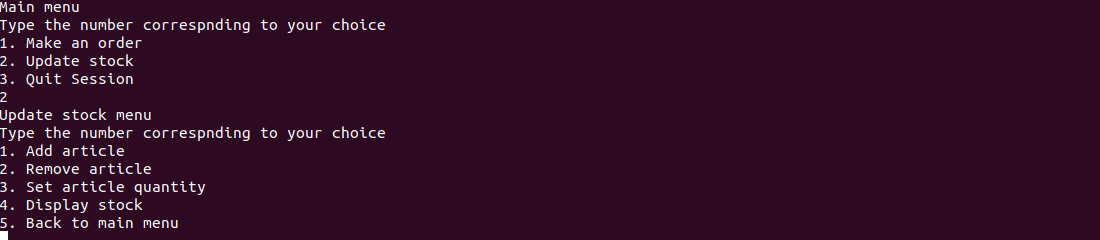
\includegraphics[scale=0.3]{captures/g_it3_11.png}
\end{center} 

\paragraph{\textbf{Option 1:}} C’est pour ajouter un nouvel article dans le stock en lui attribuant un nom au choix.
\begin{center}
	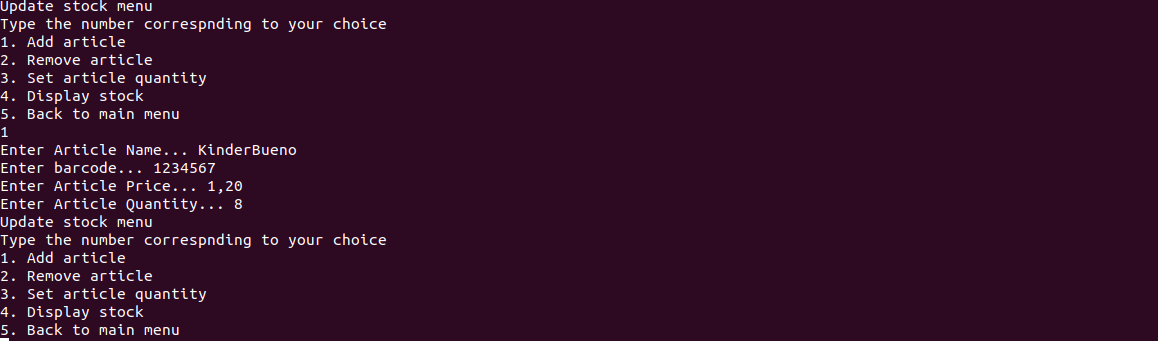
\includegraphics[scale=0.28]{captures/g_it3_12.png}
\end{center} 

\paragraph{\textbf{Option 2:}}    Elle supprime un article du stock en lui insérant son code barre.
\begin{center}
	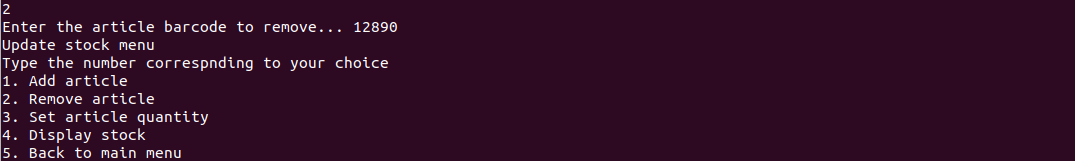
\includegraphics[scale=0.3]{captures/g_it3_13.png}
\end{center} 

\paragraph{\textbf{Option 3:}}  Elle sert à modifier la quantité des articles.
\begin{center}
	\includegraphics[scale=0.26]{captures/g_it3_15.png}
\end{center} 
L’option 3 du menu principal quitte le programme, comme figuré ci-dessous :

\paragraph{\textbf{Option 4:}}  Elle affiche les articles existant dans le stock avec toutes les informations : prix, quantité...
\begin{center}
	\includegraphics[scale=0.27]{captures/g_it3_14.png}
\end{center} 


\section{\textcolor{rr}{Itération 4}}
\subsection{\textcolor{bb}{Phase de conception}}
Le logiciel est répartir en paquetages :
\begin{itemize}
\item \textbf{ihm :} correspond au View (JSP-JLSTL, CSS, JAVASCRIPT).
\item \textbf{persistance :} daos (DAO : DATA ACCESS OBJECT) peut gère plusieurs moteur de base de données de notre cas MySQL.
\item \textbf{metier :}  beans correspond au Model.
\item \textbf{erreur :} exception.
\item \textbf{forms :} vérification des formulaires.
\item \textbf{servlets:} comme contrôleur.
\end{itemize}
\subsection{\textcolor{bb}{Phase d'implémentation}}
Les cas d'utilisation implémenter sont :
\begin{itemize}
\item Passer une commande. 
\item Gérer le stock (modifier,ajouter et supprimer.
\end{itemize}
\subsubsection{I- Interface web JEE :}
\textbf{I-1- Cas d'utilisation gérer le stock (ajouter, modifier et supprime) :}
\begin{center}
	\includegraphics[scale=0.15]{captures/1.png}
	\captionof{figure}{Accueil de l'application}
\end{center}
\begin{center}
	\includegraphics[scale=0.15]{captures/2.png}
	\captionof{figure}{Menu session gestionnaire}	
\end{center}
\begin{center}
	\includegraphics[scale=0.15]{captures/3.png}
	\captionof{figure}{Menu affichage du stock}	
\end{center}
\begin{center}
	\includegraphics[scale=0.15]{captures/4.png}
	\captionof{figure}{Menu ajouter un article}	
\end{center}
\begin{center}
	\includegraphics[scale=0.15]{captures/5.png}
	\captionof{figure}{Menu modifier un article}	
\end{center}
\textbf{I-2- Cas d'utilisation passer une commande :}
\begin{center}
	\includegraphics[scale=0.15]{captures/6.png}
	\captionof{figure}{Menu Commande}	
\end{center}
\begin{center}
	\includegraphics[scale=0.15]{captures/7.png}
	\captionof{figure}{Menu panier (ajouter, modifier et supprimer)}	
\end{center}
\begin{center}
	\includegraphics[scale=0.15]{captures/8.png}
	\captionof{figure}{Menu valider une commande(génération de la facture en pdf)}	
\end{center}
\textbf{I-3- La persistance :}
\begin{center}
	\includegraphics[scale=0.3]{captures/9.png}
	\captionof{figure}{Les tables SQL utilisées (PHP MyAdmin)}	
\end{center}
\begin{center}
	\includegraphics[scale=0.4]{captures/article.png}
	\captionof{figure}{La table Article}	
\end{center}
\begin{center}
	\includegraphics[scale=0.36]{captures/command.png}
	\captionof{figure}{La table Command}	
\end{center}
\begin{center}
	\includegraphics[scale=0.4]{captures/stock.png}
	\captionof{figure}{La table Stock}	
\end{center}

\subsubsection{II- Interface Java Swing :}
\textbf{II-1 Cas d'utilisation passer une commande :}
\begin{center}
	\includegraphics[scale=0.4]{captures/1_swing.png}
	\captionof{figure}{Menu d’accueil de l'application}	
\end{center}
\begin{center}
	\includegraphics[scale=0.4]{captures/2_swing.png}
	\captionof{figure}{Menu session de caisse}	
\end{center}
\begin{center}
	\includegraphics[scale=0.4]{captures/3_swing.png}
	\captionof{figure}{Menu Ajouter,modifier,supprimer, annuler et valider une commande}	
\end{center}
\textbf{II-2- Cas d'utilisation gérer le stock :}
\begin{center}
	\includegraphics[scale=0.4]{captures/4_swing.png}
	\captionof{figure}{Menu session gestionnaire}	
\end{center}
\begin{center}
	\includegraphics[scale=0.4]{captures/5_swing.png}
	\captionof{figure}{Menu ajouter un article}	
\end{center}
\begin{center}
	\includegraphics[scale=0.4]{captures/6_swing.png}
	\captionof{figure}{Menu supprimer un article}	
\end{center}
\begin{center}
	\includegraphics[scale=0.4]{captures/7_swing.png}
	\captionof{figure}{Menu modifier un article}	
\end{center}
\begin{center}
	\includegraphics[scale=0.2]{captures/8_swing.png}
	\captionof{figure}{le tick de caisse est généré en pdf}	
\end{center}


\section{Conclusion :}
Dans Le Cadre de ce cours on a pu acquérir plusieurs connaissance notamment : 
\begin{itemize}
\item Modalisation UML.
\item Programation java en générale.
\item Presistance : Sérialisation, MySQL, JPA.
\item Architecture MVC.
\item JEE.
\item Swing.
\end{itemize}
\textbf{\textit{Nous vous remercions d'avoir enrichi nos connaissances et de nous avoir guidé durant toute cette année.}}
\end{document}